\documentclass[twoside]{book}

% Packages required by doxygen
\usepackage{fixltx2e}
\usepackage{calc}
\usepackage{doxygen}
\usepackage[export]{adjustbox} % also loads graphicx
\usepackage{graphicx}
\usepackage[utf8]{inputenc}
\usepackage{makeidx}
\usepackage{multicol}
\usepackage{multirow}
\PassOptionsToPackage{warn}{textcomp}
\usepackage{textcomp}
\usepackage[nointegrals]{wasysym}
\usepackage[table]{xcolor}

% Font selection
\usepackage[T1]{fontenc}
\usepackage[scaled=.90]{helvet}
\usepackage{courier}
\usepackage{amssymb}
\usepackage{sectsty}
\renewcommand{\familydefault}{\sfdefault}
\allsectionsfont{%
  \fontseries{bc}\selectfont%
  \color{darkgray}%
}
\renewcommand{\DoxyLabelFont}{%
  \fontseries{bc}\selectfont%
  \color{darkgray}%
}
\newcommand{\+}{\discretionary{\mbox{\scriptsize$\hookleftarrow$}}{}{}}

% Page & text layout
\usepackage{geometry}
\geometry{%
  a4paper,%
  top=2.5cm,%
  bottom=2.5cm,%
  left=2.5cm,%
  right=2.5cm%
}
\tolerance=750
\hfuzz=15pt
\hbadness=750
\setlength{\emergencystretch}{15pt}
\setlength{\parindent}{0cm}
\setlength{\parskip}{3ex plus 2ex minus 2ex}
\makeatletter
\renewcommand{\paragraph}{%
  \@startsection{paragraph}{4}{0ex}{-1.0ex}{1.0ex}{%
    \normalfont\normalsize\bfseries\SS@parafont%
  }%
}
\renewcommand{\subparagraph}{%
  \@startsection{subparagraph}{5}{0ex}{-1.0ex}{1.0ex}{%
    \normalfont\normalsize\bfseries\SS@subparafont%
  }%
}
\makeatother

% Headers & footers
\usepackage{fancyhdr}
\pagestyle{fancyplain}
\fancyhead[LE]{\fancyplain{}{\bfseries\thepage}}
\fancyhead[CE]{\fancyplain{}{}}
\fancyhead[RE]{\fancyplain{}{\bfseries\leftmark}}
\fancyhead[LO]{\fancyplain{}{\bfseries\rightmark}}
\fancyhead[CO]{\fancyplain{}{}}
\fancyhead[RO]{\fancyplain{}{\bfseries\thepage}}
\fancyfoot[LE]{\fancyplain{}{}}
\fancyfoot[CE]{\fancyplain{}{}}
\fancyfoot[RE]{\fancyplain{}{\bfseries\scriptsize Generated by Doxygen }}
\fancyfoot[LO]{\fancyplain{}{\bfseries\scriptsize Generated by Doxygen }}
\fancyfoot[CO]{\fancyplain{}{}}
\fancyfoot[RO]{\fancyplain{}{}}
\renewcommand{\footrulewidth}{0.4pt}
\renewcommand{\chaptermark}[1]{%
  \markboth{#1}{}%
}
\renewcommand{\sectionmark}[1]{%
  \markright{\thesection\ #1}%
}

% Indices & bibliography
\usepackage{natbib}
\usepackage[titles]{tocloft}
\setcounter{tocdepth}{3}
\setcounter{secnumdepth}{5}
\makeindex

% Hyperlinks (required, but should be loaded last)
\usepackage{ifpdf}
\ifpdf
  \usepackage[pdftex,pagebackref=true]{hyperref}
\else
  \usepackage[ps2pdf,pagebackref=true]{hyperref}
\fi
\hypersetup{%
  colorlinks=true,%
  linkcolor=blue,%
  citecolor=blue,%
  unicode%
}

% Custom commands
\newcommand{\clearemptydoublepage}{%
  \newpage{\pagestyle{empty}\cleardoublepage}%
}

\usepackage{caption}
\captionsetup{labelsep=space,justification=centering,font={bf},singlelinecheck=off,skip=4pt,position=top}

%===== C O N T E N T S =====

\begin{document}

% Titlepage & ToC
\hypersetup{pageanchor=false,
             bookmarksnumbered=true,
             pdfencoding=unicode
            }
\pagenumbering{alph}
\begin{titlepage}
\vspace*{7cm}
\begin{center}%
{\Large Simple\+Game\+Engine \\[1ex]\large 1.\+0 }\\
\vspace*{1cm}
{\large Generated by Doxygen 1.8.13}\\
\end{center}
\end{titlepage}
\clearemptydoublepage
\pagenumbering{roman}
\tableofcontents
\clearemptydoublepage
\pagenumbering{arabic}
\hypersetup{pageanchor=true}

%--- Begin generated contents ---
\chapter{Hierarchical Index}
\section{Class Hierarchy}
This inheritance list is sorted roughly, but not completely, alphabetically\+:\begin{DoxyCompactList}
\item \contentsline{section}{Abstract\+Game\+Object}{\pageref{class_abstract_game_object}}{}
\begin{DoxyCompactList}
\item \contentsline{section}{Simple\+Object}{\pageref{class_simple_object}}{}
\begin{DoxyCompactList}
\item \contentsline{section}{Physical\+Object}{\pageref{class_physical_object}}{}
\end{DoxyCompactList}
\end{DoxyCompactList}
\item \contentsline{section}{Behaviour}{\pageref{class_behaviour}}{}
\begin{DoxyCompactList}
\item \contentsline{section}{Particle\+Effect}{\pageref{class_particle_effect}}{}
\end{DoxyCompactList}
\item \contentsline{section}{Camera}{\pageref{class_camera}}{}
\item \contentsline{section}{Game}{\pageref{class_game}}{}
\begin{DoxyCompactList}
\item \contentsline{section}{Example\+Game}{\pageref{class_example_game}}{}
\end{DoxyCompactList}
\item \contentsline{section}{Nk\+Window}{\pageref{class_nk_window}}{}
\item \contentsline{section}{Options}{\pageref{class_options}}{}
\item \contentsline{section}{Particle}{\pageref{struct_particle}}{}
\item \contentsline{section}{Physics\+World}{\pageref{class_physics_world}}{}
\item \contentsline{section}{Resource\+Manager}{\pageref{class_resource_manager}}{}
\item \contentsline{section}{Rigid\+Body\+Simple\+Factory}{\pageref{class_rigid_body_simple_factory}}{}
\item \contentsline{section}{Shader}{\pageref{class_shader}}{}
\item \contentsline{section}{Texture}{\pageref{class_texture}}{}
\item \contentsline{section}{Vao\+Object}{\pageref{class_vao_object}}{}
\end{DoxyCompactList}

\chapter{Class Index}
\section{Class List}
Here are the classes, structs, unions and interfaces with brief descriptions\+:\begin{DoxyCompactList}
\item\contentsline{section}{\hyperlink{class_abstract_game_object}{Abstract\+Game\+Object} \\*Abstrakcyjna klasa definiujaca interfejs dla obiektow w grze. Jej implementacje mozna znalesc w klasach \hyperlink{class_physical_object}{Physical\+Object} oraz \hyperlink{class_simple_object}{Simple\+Object}. /summary$>$ }{\pageref{class_abstract_game_object}}{}
\item\contentsline{section}{\hyperlink{class_behaviour}{Behaviour} \\*abstrakcyjna klasa ktora miala miec mozliwosc dodawania dodatkowych zachowan do obiektow. Nie doczekala sie swojej implementacji. }{\pageref{class_behaviour}}{}
\item\contentsline{section}{\hyperlink{class_camera}{Camera} \\*klasa reprezetujaca obiekt kamery z ktorej pozycji uzytkownik widzi swiat gry }{\pageref{class_camera}}{}
\item\contentsline{section}{\hyperlink{class_example_game}{Example\+Game} \\*klasa rozszerzajaca klase \hyperlink{class_game}{Game}. posiada metody inicjalizujace poczatkowy stan oraz inicjalizacje zasobow }{\pageref{class_example_game}}{}
\item\contentsline{section}{\hyperlink{class_game}{Game} }{\pageref{class_game}}{}
\item\contentsline{section}{\hyperlink{class_nk_window}{Nk\+Window} \\*klasa przedstawiajaca okno opcji w grze. /summary$>$ }{\pageref{class_nk_window}}{}
\item\contentsline{section}{\hyperlink{class_options}{Options} \\*klasa przedstawiajaca opcje w grze. Z jej wartosci korzysta klasa glowna gry \hyperlink{class_game}{Game}. Jest edytowana przez klase N\+Kwindow /summary$>$ }{\pageref{class_options}}{}
\item\contentsline{section}{\hyperlink{struct_particle}{Particle} \\*struktura ktora miala przechowywac dane o czasteczce wchodzacej w sklad efektu czasteczkowego }{\pageref{struct_particle}}{}
\item\contentsline{section}{\hyperlink{class_particle_effect}{Particle\+Effect} }{\pageref{class_particle_effect}}{}
\item\contentsline{section}{\hyperlink{class_physical_object}{Physical\+Object} \\*klasa rozszerzajaca klase \hyperlink{class_simple_object}{Simple\+Object} posiada dodatkowe pole opisujace ksztalt oraz wlasciwosci obiektu fizycznego /summary$>$ }{\pageref{class_physical_object}}{}
\item\contentsline{section}{\hyperlink{class_physics_world}{Physics\+World} \\*klasa reprezetujaca fizyczny swiat. /summary$>$ }{\pageref{class_physics_world}}{}
\item\contentsline{section}{\hyperlink{class_resource_manager}{Resource\+Manager} \\*statyczna klasa odpowiedzialna za wczytywanie oraz przechowywanie zasob�w takich jak tekstury , shadery oraz siatki(\+Vertex Array Objects). Klasa ta tworzy instancje klas \hyperlink{class_shader}{Shader},\hyperlink{class_texture}{Texture} i \hyperlink{class_vao_object}{Vao\+Object}. /summary$>$ }{\pageref{class_resource_manager}}{}
\item\contentsline{section}{\hyperlink{class_rigid_body_simple_factory}{Rigid\+Body\+Simple\+Factory} \\*klasa odpowiadajaca za tworzenie cial fizycznych /summary$>$ }{\pageref{class_rigid_body_simple_factory}}{}
\item\contentsline{section}{\hyperlink{class_shader}{Shader} \\*klasa umo�liwiaj�ca kompilacje shaderow. Przechowywane w polu numer ID shadera. Posiada metod� use() kt�ra wywo�uje funkcj� gl\+Use\+Program dla ID przechowywanego w polu obiektu }{\pageref{class_shader}}{}
\item\contentsline{section}{\hyperlink{class_simple_object}{Simple\+Object} \\*klasa implementujaca \hyperlink{class_abstract_game_object}{Abstract\+Game\+Object}. Reprezetuje podstawowy obiekt gry nie posiadajacy wlasciwosci fizycznych /summary$>$ }{\pageref{class_simple_object}}{}
\item\contentsline{section}{\hyperlink{class_texture}{Texture} \\*Klasa umo�liwiaj�ca generowanie tekstury na podstawie obrazu. Przechowywuj� w polu ID tekstury oraz informacje o teksturze takie jak rozmiar, wrap, filter. /summary$>$ }{\pageref{class_texture}}{}
\item\contentsline{section}{\hyperlink{class_vao_object}{Vao\+Object} \\*Klasa ta umo�liwia generowanie Vao na podstawie tablicy wierzcho�k�w. W tablicy wierzcho�k�w przechowywane s� ich wsp�rz�dne, wsp�rz�dne tekstur oraz opcjonalnie normalne wierzcho�k�w. Klasa posiada pole przechowuj�ce id wygenerowanego V\+AO.}{\pageref{class_vao_object}}{}
\end{DoxyCompactList}

\chapter{Class Documentation}
\hypertarget{class_abstract_game_object}{}\section{Abstract\+Game\+Object Class Reference}
\label{class_abstract_game_object}\index{Abstract\+Game\+Object@{Abstract\+Game\+Object}}


Abstrakcyjna klasa definiujaca interfejs dla obiektow w grze. Jej implementacje mozna znalesc w klasach \hyperlink{class_physical_object}{Physical\+Object} oraz \hyperlink{class_simple_object}{Simple\+Object}. /summary$>$  




{\ttfamily \#include $<$Abstract\+Game\+Object.\+h$>$}

Inheritance diagram for Abstract\+Game\+Object\+:\begin{figure}[H]
\begin{center}
\leavevmode
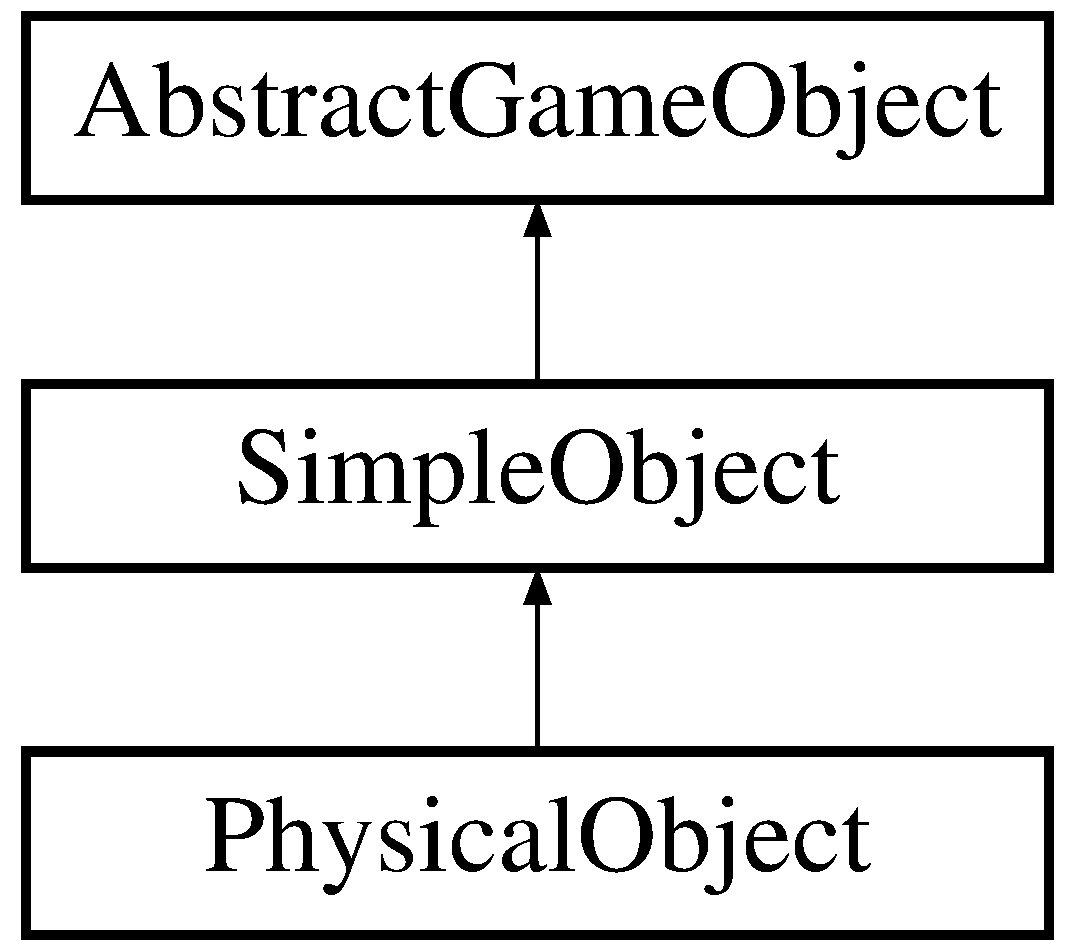
\includegraphics[height=3.000000cm]{class_abstract_game_object}
\end{center}
\end{figure}
\subsection*{Public Member Functions}
\begin{DoxyCompactItemize}
\item 
\hyperlink{class_abstract_game_object_aaf1bae3e1afb1b7269122466d41cb350}{$\sim$\+Abstract\+Game\+Object} ()
\item 
\mbox{\Hypertarget{class_abstract_game_object_aeec87788c72b2492040917cabb7f5c6e}\label{class_abstract_game_object_aeec87788c72b2492040917cabb7f5c6e}} 
virtual void {\bfseries set\+Position} (glm\+::vec3 position)=0
\item 
virtual glm\+::vec3 \hyperlink{class_abstract_game_object_ac934d513fd18a520d8b68dd5a7ac7399}{get\+Position} ()=0
\item 
virtual void \hyperlink{class_abstract_game_object_a162f800603ac5671ff24ad8042c062b5}{update} ()=0
\item 
\mbox{\Hypertarget{class_abstract_game_object_a77d713fdeeed8310e4152dbf352d988e}\label{class_abstract_game_object_a77d713fdeeed8310e4152dbf352d988e}} 
virtual void {\bfseries draw} ()=0
\item 
\mbox{\Hypertarget{class_abstract_game_object_a4688b8a17299804d82c99160851b68ce}\label{class_abstract_game_object_a4688b8a17299804d82c99160851b68ce}} 
virtual void {\bfseries set\+Visible} (bool visible)=0
\item 
virtual bool \hyperlink{class_abstract_game_object_afddc4040f2d1a7effc0e0baa9950b2e2}{is\+Visible} ()=0
\item 
\mbox{\Hypertarget{class_abstract_game_object_a1fdfaf1362c1635965dd194d7f22743c}\label{class_abstract_game_object_a1fdfaf1362c1635965dd194d7f22743c}} 
virtual void {\bfseries to\+Xml} (X\+M\+L\+Document $\ast$xml\+Doc)=0
\end{DoxyCompactItemize}
\subsection*{Protected Attributes}
\begin{DoxyCompactItemize}
\item 
\mbox{\Hypertarget{class_abstract_game_object_a3a116439cb78825f98b1252746d16dc0}\label{class_abstract_game_object_a3a116439cb78825f98b1252746d16dc0}} 
bool {\bfseries visible}
\end{DoxyCompactItemize}


\subsection{Detailed Description}
Abstrakcyjna klasa definiujaca interfejs dla obiektow w grze. Jej implementacje mozna znalesc w klasach \hyperlink{class_physical_object}{Physical\+Object} oraz \hyperlink{class_simple_object}{Simple\+Object}. /summary$>$ 

\subsection{Constructor \& Destructor Documentation}
\mbox{\Hypertarget{class_abstract_game_object_aaf1bae3e1afb1b7269122466d41cb350}\label{class_abstract_game_object_aaf1bae3e1afb1b7269122466d41cb350}} 
\index{Abstract\+Game\+Object@{Abstract\+Game\+Object}!````~Abstract\+Game\+Object@{$\sim$\+Abstract\+Game\+Object}}
\index{````~Abstract\+Game\+Object@{$\sim$\+Abstract\+Game\+Object}!Abstract\+Game\+Object@{Abstract\+Game\+Object}}
\subsubsection{\texorpdfstring{$\sim$\+Abstract\+Game\+Object()}{~AbstractGameObject()}}
{\footnotesize\ttfamily Abstract\+Game\+Object\+::$\sim$\+Abstract\+Game\+Object (\begin{DoxyParamCaption}{ }\end{DoxyParamCaption})}

summary$>$ Metoda sluzaca do ustawiania pozycji obiektu /summary$>$ 

\subsection{Member Function Documentation}
\mbox{\Hypertarget{class_abstract_game_object_ac934d513fd18a520d8b68dd5a7ac7399}\label{class_abstract_game_object_ac934d513fd18a520d8b68dd5a7ac7399}} 
\index{Abstract\+Game\+Object@{Abstract\+Game\+Object}!get\+Position@{get\+Position}}
\index{get\+Position@{get\+Position}!Abstract\+Game\+Object@{Abstract\+Game\+Object}}
\subsubsection{\texorpdfstring{get\+Position()}{getPosition()}}
{\footnotesize\ttfamily virtual glm\+::vec3 Abstract\+Game\+Object\+::get\+Position (\begin{DoxyParamCaption}{ }\end{DoxyParamCaption})\hspace{0.3cm}{\ttfamily [pure virtual]}}

summary$>$ metoda wywolywana co klatke aktualizujaca stan obiektu /summary$>$ 

Implemented in \hyperlink{class_simple_object_acaf96b4cf35863ca69a123d9404f4e5f}{Simple\+Object}.

\mbox{\Hypertarget{class_abstract_game_object_afddc4040f2d1a7effc0e0baa9950b2e2}\label{class_abstract_game_object_afddc4040f2d1a7effc0e0baa9950b2e2}} 
\index{Abstract\+Game\+Object@{Abstract\+Game\+Object}!is\+Visible@{is\+Visible}}
\index{is\+Visible@{is\+Visible}!Abstract\+Game\+Object@{Abstract\+Game\+Object}}
\subsubsection{\texorpdfstring{is\+Visible()}{isVisible()}}
{\footnotesize\ttfamily virtual bool Abstract\+Game\+Object\+::is\+Visible (\begin{DoxyParamCaption}{ }\end{DoxyParamCaption})\hspace{0.3cm}{\ttfamily [pure virtual]}}

summary$>$ metoda dodajaca fragment bedacy opisem obiektu jako X\+ML do dokumentu na ktory wskaznik podawany jest w parametrze /summary$>$ 

Implemented in \hyperlink{class_simple_object_a2475d0a90f1cb7bc5765a632efe9ddd4}{Simple\+Object}.

\mbox{\Hypertarget{class_abstract_game_object_a162f800603ac5671ff24ad8042c062b5}\label{class_abstract_game_object_a162f800603ac5671ff24ad8042c062b5}} 
\index{Abstract\+Game\+Object@{Abstract\+Game\+Object}!update@{update}}
\index{update@{update}!Abstract\+Game\+Object@{Abstract\+Game\+Object}}
\subsubsection{\texorpdfstring{update()}{update()}}
{\footnotesize\ttfamily virtual void Abstract\+Game\+Object\+::update (\begin{DoxyParamCaption}{ }\end{DoxyParamCaption})\hspace{0.3cm}{\ttfamily [pure virtual]}}

summary$>$ metoda wywolywana co klatke rysujaca obiekt na ekranie /summary$>$ 

Implemented in \hyperlink{class_physical_object_a3005ac0afce838049101db17525f6004}{Physical\+Object}, and \hyperlink{class_simple_object_a38a3ceafd11a673fd68dd87ed6ebd35b}{Simple\+Object}.



The documentation for this class was generated from the following files\+:\begin{DoxyCompactItemize}
\item 
C\+:/\+Users/szymk/\+Downloads/\+Nowy folder/\+Simple\+Game\+Engine/\+Simple\+Game\+Engine/\+G\+Kp/Abstract\+Game\+Object.\+h\item 
C\+:/\+Users/szymk/\+Downloads/\+Nowy folder/\+Simple\+Game\+Engine/\+Simple\+Game\+Engine/\+G\+Kp/Abstract\+Game\+Object.\+cpp\end{DoxyCompactItemize}

\hypertarget{class_behaviour}{}\section{Behaviour Class Reference}
\label{class_behaviour}\index{Behaviour@{Behaviour}}


abstrakcyjna klasa ktora miala miec mozliwosc dodawania dodatkowych zachowan do obiektow. Nie doczekala sie swojej implementacji.  




{\ttfamily \#include $<$Behaviour.\+h$>$}

Inheritance diagram for Behaviour\+:\begin{figure}[H]
\begin{center}
\leavevmode
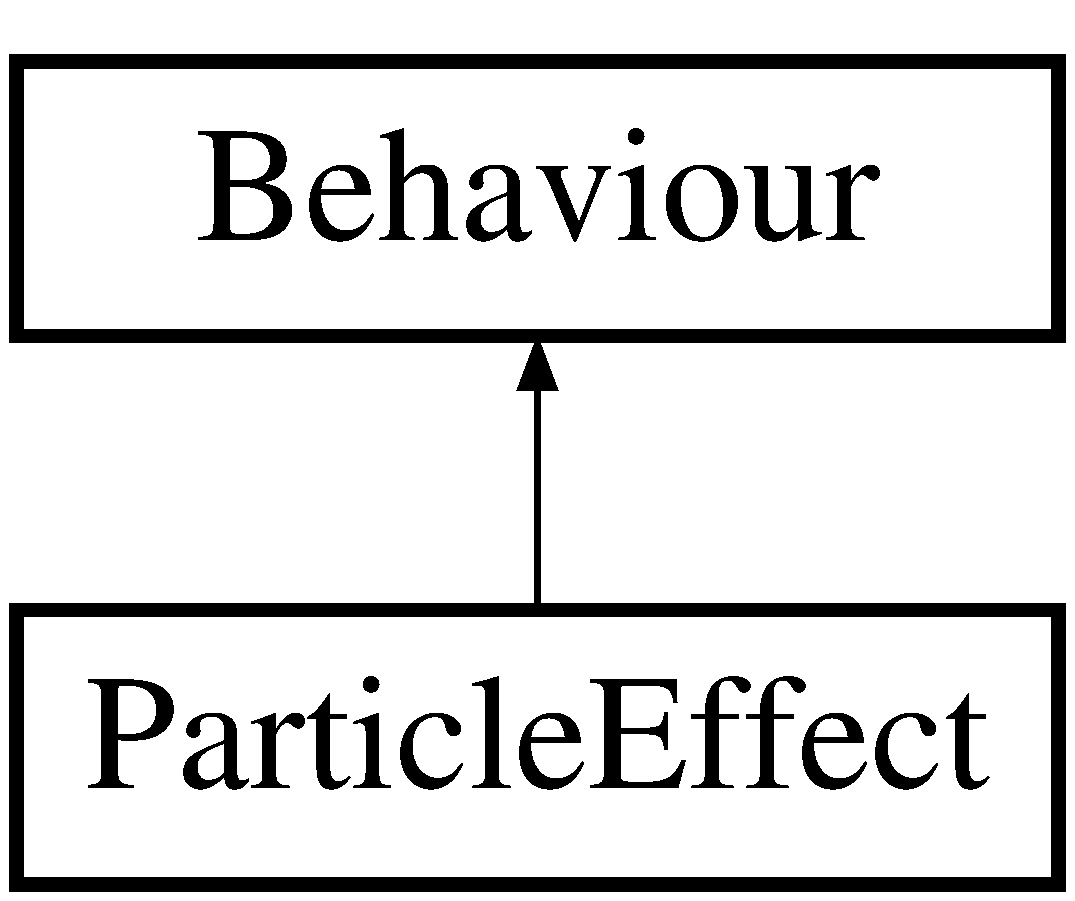
\includegraphics[height=2.000000cm]{class_behaviour}
\end{center}
\end{figure}
\subsection*{Public Member Functions}
\begin{DoxyCompactItemize}
\item 
\mbox{\Hypertarget{class_behaviour_ac7dfbc3199c2ebb1fd7d845ebb751117}\label{class_behaviour_ac7dfbc3199c2ebb1fd7d845ebb751117}} 
virtual void {\bfseries set\+Root} (\hyperlink{class_abstract_game_object}{Abstract\+Game\+Object} $\ast$object)
\item 
\mbox{\Hypertarget{class_behaviour_ac88cef5429abdbc3809f8ee545613dcb}\label{class_behaviour_ac88cef5429abdbc3809f8ee545613dcb}} 
virtual void {\bfseries update} ()=0
\item 
\mbox{\Hypertarget{class_behaviour_a94724613d5c4651c8177d77c7808612c}\label{class_behaviour_a94724613d5c4651c8177d77c7808612c}} 
virtual void {\bfseries init} ()=0
\end{DoxyCompactItemize}
\subsection*{Protected Attributes}
\begin{DoxyCompactItemize}
\item 
\mbox{\Hypertarget{class_behaviour_a302037bf6f38ca4b28e061cbdeb61b64}\label{class_behaviour_a302037bf6f38ca4b28e061cbdeb61b64}} 
\hyperlink{class_abstract_game_object}{Abstract\+Game\+Object} $\ast$ {\bfseries root}
\end{DoxyCompactItemize}


\subsection{Detailed Description}
abstrakcyjna klasa ktora miala miec mozliwosc dodawania dodatkowych zachowan do obiektow. Nie doczekala sie swojej implementacji. 



The documentation for this class was generated from the following files\+:\begin{DoxyCompactItemize}
\item 
C\+:/\+Users/szymk/\+Downloads/\+Nowy folder/\+Simple\+Game\+Engine/\+Simple\+Game\+Engine/\+G\+Kp/Behaviour.\+h\item 
C\+:/\+Users/szymk/\+Downloads/\+Nowy folder/\+Simple\+Game\+Engine/\+Simple\+Game\+Engine/\+G\+Kp/Behaviour.\+cpp\end{DoxyCompactItemize}

\hypertarget{class_camera}{}\section{Camera Class Reference}
\label{class_camera}\index{Camera@{Camera}}


klasa reprezetujaca obiekt kamery z ktorej pozycji uzytkownik widzi swiat gry  




{\ttfamily \#include $<$Camera.\+h$>$}

\subsection*{Public Member Functions}
\begin{DoxyCompactItemize}
\item 
\mbox{\Hypertarget{class_camera_ad81c45f1ffb7af4fc5e9299721ebfcf7}\label{class_camera_ad81c45f1ffb7af4fc5e9299721ebfcf7}} 
{\bfseries Camera} (glm\+::vec3 position=D\+E\+F\+A\+U\+L\+T\+\_\+\+P\+O\+S\+I\+T\+I\+ON, glm\+::vec3 up=D\+E\+F\+A\+U\+L\+T\+\_\+\+W\+O\+R\+L\+D\+\_\+\+UP, G\+Lfloat yaw=D\+E\+F\+A\+U\+L\+T\+\_\+\+Y\+AW, G\+Lfloat pitch=D\+E\+F\+A\+U\+L\+T\+\_\+\+P\+I\+T\+CH)
\item 
\mbox{\Hypertarget{class_camera_affa333055635aed96518c4c66be9a70c}\label{class_camera_affa333055635aed96518c4c66be9a70c}} 
glm\+::mat4 {\bfseries Get\+View\+Matrix} ()
\item 
void \hyperlink{class_camera_a42cda7239981a5618660d04bd5893556}{update} ()
\begin{DoxyCompactList}\small\item\em metoda wywolywana co klatke. aktualizuje wektory kamery oraz jej pozycje \end{DoxyCompactList}\item 
void \hyperlink{class_camera_a79693c3d7c085b0252216f8348b525ce}{move\+Forward} (G\+Lfloat value)
\begin{DoxyCompactList}\small\item\em przemieszcza kamere do przodu (wartosc ujemna przemieszcza do tylu) \end{DoxyCompactList}\item 
void \hyperlink{class_camera_ac0f82a424f190cc4f65e5f485d2317d2}{move\+Right} (G\+Lfloat value)
\item 
void \hyperlink{class_camera_a945b9054e8f7f840d29bff164cf57f65}{move\+Up} (G\+Lfloat value)
\item 
\mbox{\Hypertarget{class_camera_aad3c6e5fa354cd87ee7404092f21cc66}\label{class_camera_aad3c6e5fa354cd87ee7404092f21cc66}} 
void {\bfseries rotate\+Camera} (G\+Lfloat x, G\+Lfloat y)
\item 
glm\+::vec3 \hyperlink{class_camera_ab40fb75b3d34a86d92fff61bb1675097}{get\+Pos} ()
\item 
\mbox{\Hypertarget{class_camera_a3da785a7091a11554a63b7ef387ee317}\label{class_camera_a3da785a7091a11554a63b7ef387ee317}} 
glm\+::vec3 {\bfseries getfront} ()
\end{DoxyCompactItemize}


\subsection{Detailed Description}
klasa reprezetujaca obiekt kamery z ktorej pozycji uzytkownik widzi swiat gry 



\subsection{Member Function Documentation}
\mbox{\Hypertarget{class_camera_ab40fb75b3d34a86d92fff61bb1675097}\label{class_camera_ab40fb75b3d34a86d92fff61bb1675097}} 
\index{Camera@{Camera}!get\+Pos@{get\+Pos}}
\index{get\+Pos@{get\+Pos}!Camera@{Camera}}
\subsubsection{\texorpdfstring{get\+Pos()}{getPos()}}
{\footnotesize\ttfamily glm\+::vec3 Camera\+::get\+Pos (\begin{DoxyParamCaption}{ }\end{DoxyParamCaption})}

summary$>$ pobiera wektor wskazujacy kierunek skierowania kamery /summary$>$ \mbox{\Hypertarget{class_camera_a79693c3d7c085b0252216f8348b525ce}\label{class_camera_a79693c3d7c085b0252216f8348b525ce}} 
\index{Camera@{Camera}!move\+Forward@{move\+Forward}}
\index{move\+Forward@{move\+Forward}!Camera@{Camera}}
\subsubsection{\texorpdfstring{move\+Forward()}{moveForward()}}
{\footnotesize\ttfamily void Camera\+::move\+Forward (\begin{DoxyParamCaption}\item[{G\+Lfloat}]{value }\end{DoxyParamCaption})}



przemieszcza kamere do przodu (wartosc ujemna przemieszcza do tylu) 

summary$>$ przemieszcza kamere w prawo (podanie wartosci ujemnej przemieszcza w lewo) /summary$>$ \mbox{\Hypertarget{class_camera_ac0f82a424f190cc4f65e5f485d2317d2}\label{class_camera_ac0f82a424f190cc4f65e5f485d2317d2}} 
\index{Camera@{Camera}!move\+Right@{move\+Right}}
\index{move\+Right@{move\+Right}!Camera@{Camera}}
\subsubsection{\texorpdfstring{move\+Right()}{moveRight()}}
{\footnotesize\ttfamily void Camera\+::move\+Right (\begin{DoxyParamCaption}\item[{G\+Lfloat}]{value }\end{DoxyParamCaption})}

summary$>$ przemieszcza kamere do gory (lub w dol dla wartosci ujemnej) /summary$>$ \mbox{\Hypertarget{class_camera_a945b9054e8f7f840d29bff164cf57f65}\label{class_camera_a945b9054e8f7f840d29bff164cf57f65}} 
\index{Camera@{Camera}!move\+Up@{move\+Up}}
\index{move\+Up@{move\+Up}!Camera@{Camera}}
\subsubsection{\texorpdfstring{move\+Up()}{moveUp()}}
{\footnotesize\ttfamily void Camera\+::move\+Up (\begin{DoxyParamCaption}\item[{G\+Lfloat}]{value }\end{DoxyParamCaption})}

summary$>$ obraca kamere /summary$>$ \mbox{\Hypertarget{class_camera_a42cda7239981a5618660d04bd5893556}\label{class_camera_a42cda7239981a5618660d04bd5893556}} 
\index{Camera@{Camera}!update@{update}}
\index{update@{update}!Camera@{Camera}}
\subsubsection{\texorpdfstring{update()}{update()}}
{\footnotesize\ttfamily void Camera\+::update (\begin{DoxyParamCaption}{ }\end{DoxyParamCaption})}



metoda wywolywana co klatke. aktualizuje wektory kamery oraz jej pozycje 



The documentation for this class was generated from the following files\+:\begin{DoxyCompactItemize}
\item 
C\+:/\+Users/szymk/\+Downloads/\+Nowy folder/\+Simple\+Game\+Engine/\+Simple\+Game\+Engine/\+G\+Kp/Camera.\+h\item 
C\+:/\+Users/szymk/\+Downloads/\+Nowy folder/\+Simple\+Game\+Engine/\+Simple\+Game\+Engine/\+G\+Kp/Camera.\+cpp\end{DoxyCompactItemize}

\hypertarget{class_example_game}{}\section{Example\+Game Class Reference}
\label{class_example_game}\index{Example\+Game@{Example\+Game}}


klasa rozszerzajaca klase \hyperlink{class_game}{Game}. posiada metody inicjalizujace poczatkowy stan oraz inicjalizacje zasobow  




{\ttfamily \#include $<$Example\+Game.\+h$>$}

Inheritance diagram for Example\+Game\+:\begin{figure}[H]
\begin{center}
\leavevmode
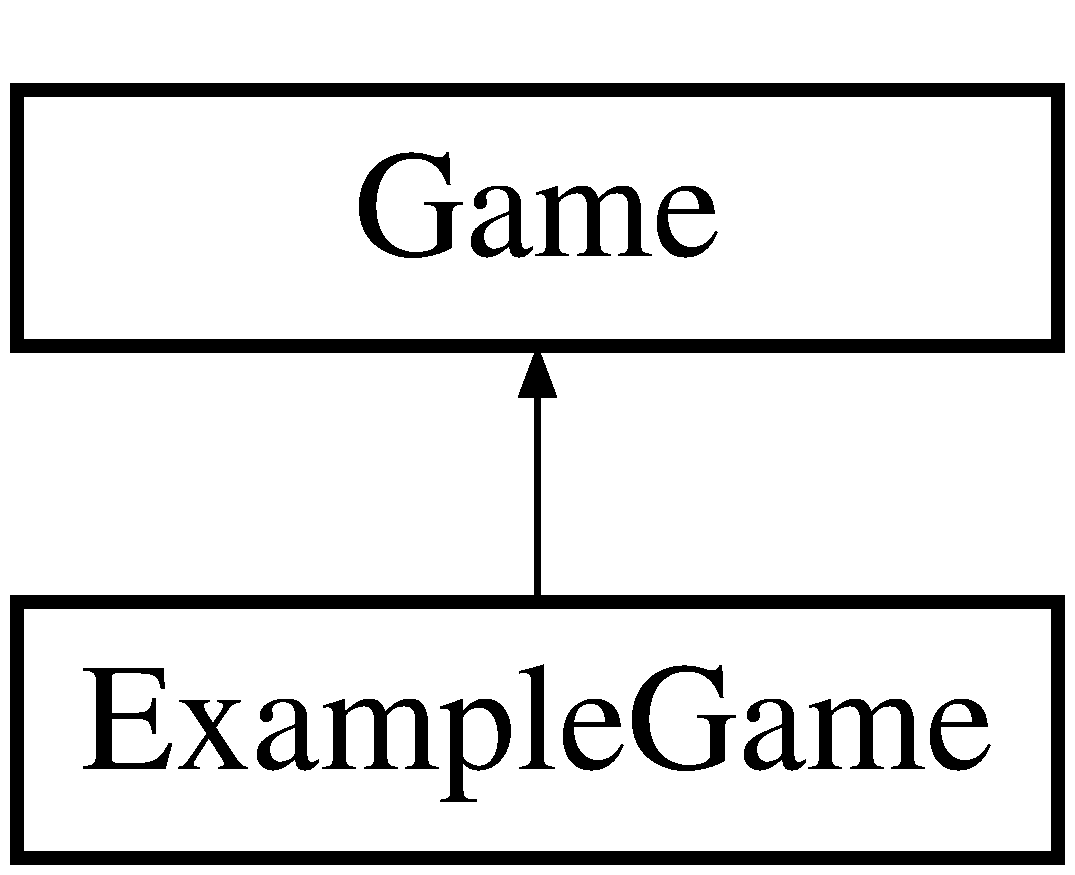
\includegraphics[height=2.000000cm]{class_example_game}
\end{center}
\end{figure}
\subsection*{Public Member Functions}
\begin{DoxyCompactItemize}
\item 
\mbox{\Hypertarget{class_example_game_adb33bb2a79998a43a0341e2aacf0e6c7}\label{class_example_game_adb33bb2a79998a43a0341e2aacf0e6c7}} 
{\bfseries Example\+Game} (G\+L\+F\+Wwindow $\ast$window)
\item 
virtual void \hyperlink{class_example_game_ab7b84dad80cbf4eefd562f0c8e6495ab}{init} ()
\begin{DoxyCompactList}\small\item\em metoda odpowiedzialna za przygotowanie wstepnego stanu gry \end{DoxyCompactList}\end{DoxyCompactItemize}
\subsection*{Protected Member Functions}
\begin{DoxyCompactItemize}
\item 
\mbox{\Hypertarget{class_example_game_a7944aa343acdc2373bf3c4704dff2893}\label{class_example_game_a7944aa343acdc2373bf3c4704dff2893}} 
virtual void {\bfseries process\+Input} ()
\item 
\mbox{\Hypertarget{class_example_game_a16aa2ede5884f61d85b2afe07066a0e3}\label{class_example_game_a16aa2ede5884f61d85b2afe07066a0e3}} 
virtual void {\bfseries update} ()
\item 
\mbox{\Hypertarget{class_example_game_a9e44c5d059433d2726b9316ae3ba884c}\label{class_example_game_a9e44c5d059433d2726b9316ae3ba884c}} 
void {\bfseries init\+Skybox} ()
\item 
\mbox{\Hypertarget{class_example_game_a5ca873fd98a90b3c25c0699977e2faa0}\label{class_example_game_a5ca873fd98a90b3c25c0699977e2faa0}} 
void {\bfseries init\+Prototypes} ()
\item 
\mbox{\Hypertarget{class_example_game_adbc03f8b534894675bc05ca90f7c59b0}\label{class_example_game_adbc03f8b534894675bc05ca90f7c59b0}} 
void {\bfseries init\+Floor\+Plane} ()
\item 
\mbox{\Hypertarget{class_example_game_ab772e1914b60ff53a5b20c6dd1fb2894}\label{class_example_game_ab772e1914b60ff53a5b20c6dd1fb2894}} 
void {\bfseries init\+Some\+Wall} (int x, int y)
\item 
\mbox{\Hypertarget{class_example_game_a1d799ceadbd869a3c5e50512e02e3104}\label{class_example_game_a1d799ceadbd869a3c5e50512e02e3104}} 
void {\bfseries create\+Object} (glm\+::vec3 pos)
\item 
\mbox{\Hypertarget{class_example_game_a0a2bd4a82db3e4ec5af7498423e86bae}\label{class_example_game_a0a2bd4a82db3e4ec5af7498423e86bae}} 
void {\bfseries create\+Brick} (glm\+::vec3 pos)
\end{DoxyCompactItemize}
\subsection*{Protected Attributes}
\begin{DoxyCompactItemize}
\item 
\mbox{\Hypertarget{class_example_game_acb52f0540c7ebc801d21f8c7f77d7487}\label{class_example_game_acb52f0540c7ebc801d21f8c7f77d7487}} 
\hyperlink{class_simple_object}{Simple\+Object} $\ast$ {\bfseries ball2}
\end{DoxyCompactItemize}
\subsection*{Additional Inherited Members}


\subsection{Detailed Description}
klasa rozszerzajaca klase \hyperlink{class_game}{Game}. posiada metody inicjalizujace poczatkowy stan oraz inicjalizacje zasobow 



\subsection{Member Function Documentation}
\mbox{\Hypertarget{class_example_game_ab7b84dad80cbf4eefd562f0c8e6495ab}\label{class_example_game_ab7b84dad80cbf4eefd562f0c8e6495ab}} 
\index{Example\+Game@{Example\+Game}!init@{init}}
\index{init@{init}!Example\+Game@{Example\+Game}}
\subsubsection{\texorpdfstring{init()}{init()}}
{\footnotesize\ttfamily void Example\+Game\+::init (\begin{DoxyParamCaption}{ }\end{DoxyParamCaption})\hspace{0.3cm}{\ttfamily [virtual]}}



metoda odpowiedzialna za przygotowanie wstepnego stanu gry 



Reimplemented from \hyperlink{class_game_a6f3a33940524b6ba9d83f627ccb14bbf}{Game}.



The documentation for this class was generated from the following files\+:\begin{DoxyCompactItemize}
\item 
C\+:/\+Users/szymk/\+Downloads/\+Nowy folder/\+Simple\+Game\+Engine/\+Simple\+Game\+Engine/\+G\+Kp/Example\+Game.\+h\item 
C\+:/\+Users/szymk/\+Downloads/\+Nowy folder/\+Simple\+Game\+Engine/\+Simple\+Game\+Engine/\+G\+Kp/Example\+Game.\+cpp\end{DoxyCompactItemize}

\hypertarget{class_game}{}\section{Game Class Reference}
\label{class_game}\index{Game@{Game}}
Inheritance diagram for Game\+:\begin{figure}[H]
\begin{center}
\leavevmode
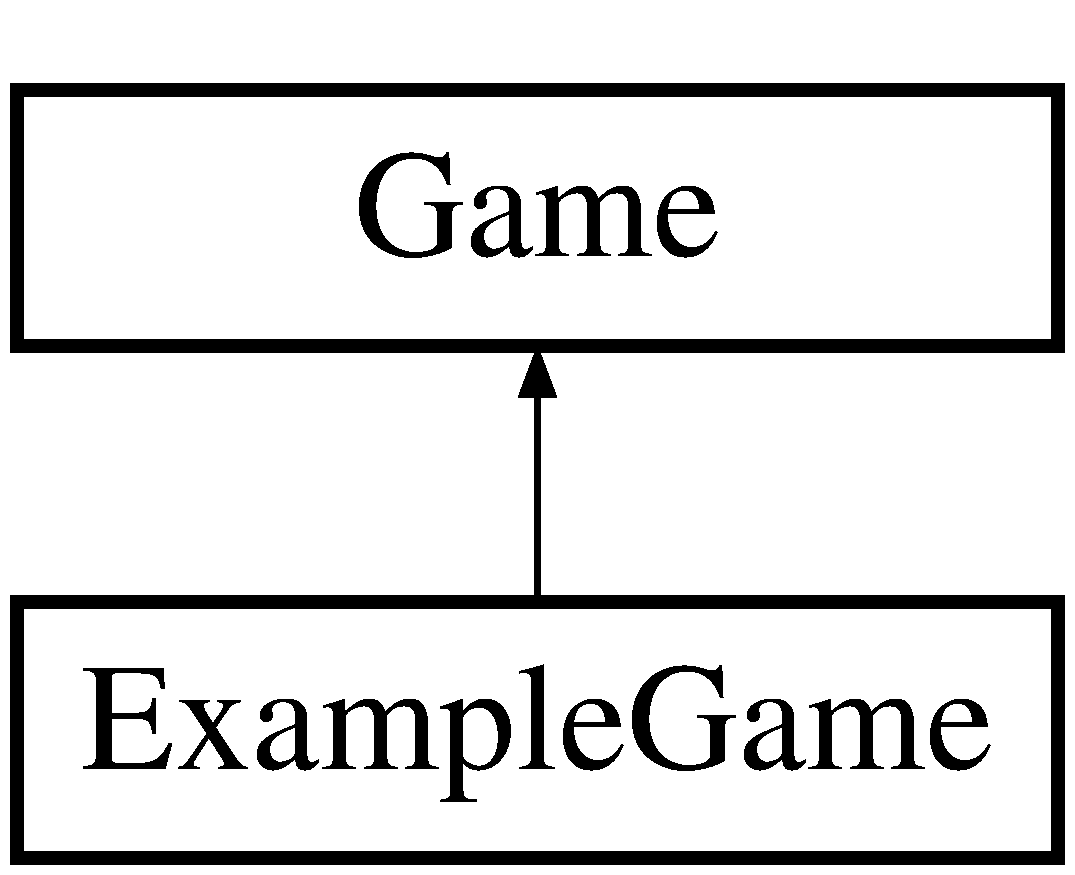
\includegraphics[height=2.000000cm]{class_game}
\end{center}
\end{figure}
\subsection*{Public Member Functions}
\begin{DoxyCompactItemize}
\item 
\mbox{\Hypertarget{class_game_aa6ff0b765ee893dfb1aa2ad1a441b227}\label{class_game_aa6ff0b765ee893dfb1aa2ad1a441b227}} 
{\bfseries Game} (G\+L\+F\+Wwindow $\ast$window)
\item 
virtual void \hyperlink{class_game_abf74d863d666bc8e1c5aa8942ba0ac18}{start\+Main\+Game\+Loop} ()
\begin{DoxyCompactList}\small\item\em metoda uruchamiajaca glowna petle gry ktora trwa az do wylaczenia programu \end{DoxyCompactList}\item 
void \hyperlink{class_game_a403da81cad9f17da729f7362768ba118}{set\+Key} (int key\+Index)
\begin{DoxyCompactList}\small\item\em metoda ustawiajaca na true flage wcisniecia klawisza o indeksie podanym w parametrze \end{DoxyCompactList}\item 
void \hyperlink{class_game_a90758cbf907d59c91ee811c45f70b654}{clear\+Key} (int key\+Index)
\begin{DoxyCompactList}\small\item\em metoda ustawiajaca na false flage wcisniecia klawisza o indeksie podanym w parametrze \end{DoxyCompactList}\item 
void \hyperlink{class_game_a62e1c1e74cccf1ecb4afe50495dfd521}{change\+Camera\+Direction} (G\+Lfloat x, G\+Lfloat y)
\begin{DoxyCompactList}\small\item\em metoda pozwalajaca na zmiane kierunku kamery \end{DoxyCompactList}\item 
virtual void \hyperlink{class_game_a6f3a33940524b6ba9d83f627ccb14bbf}{init} ()
\begin{DoxyCompactList}\small\item\em metoda odpowiedzialna za przygotowanie wstepnego stanu gry \end{DoxyCompactList}\end{DoxyCompactItemize}
\subsection*{Protected Member Functions}
\begin{DoxyCompactItemize}
\item 
\mbox{\Hypertarget{class_game_a404edbd2948699478b9d1ae7d35ee053}\label{class_game_a404edbd2948699478b9d1ae7d35ee053}} 
virtual void {\bfseries init\+Floor\+Plane} ()
\item 
\mbox{\Hypertarget{class_game_a79df6376b332d63c9eca0dcee30305c3}\label{class_game_a79df6376b332d63c9eca0dcee30305c3}} 
virtual void {\bfseries update} ()
\item 
\mbox{\Hypertarget{class_game_a15ddd769261d923827a3cdf41499c843}\label{class_game_a15ddd769261d923827a3cdf41499c843}} 
virtual void {\bfseries render} ()
\item 
\mbox{\Hypertarget{class_game_a815a3ec2787b4b1c4077d28165c380e8}\label{class_game_a815a3ec2787b4b1c4077d28165c380e8}} 
virtual void {\bfseries process\+Input} ()
\item 
\mbox{\Hypertarget{class_game_ad1945c922f49185fe91abdfb9faa4c07}\label{class_game_ad1945c922f49185fe91abdfb9faa4c07}} 
void {\bfseries exit\+Game} ()
\item 
\mbox{\Hypertarget{class_game_af996f68e716869dcb91a5ffecfd150f5}\label{class_game_af996f68e716869dcb91a5ffecfd150f5}} 
void {\bfseries generate\+Cubes} (G\+Luint x, G\+Luint y)
\item 
\mbox{\Hypertarget{class_game_a608ac4d977202eebc0327efcb1ee90c7}\label{class_game_a608ac4d977202eebc0327efcb1ee90c7}} 
void {\bfseries generate\+Tree} (G\+Luint x, G\+Luint y, G\+Luint h, G\+Luint s)
\item 
\mbox{\Hypertarget{class_game_af5aa3aaff87a42f81e334104972c3473}\label{class_game_af5aa3aaff87a42f81e334104972c3473}} 
void {\bfseries draw\+Cubes} ()
\item 
\mbox{\Hypertarget{class_game_a993305edd46b0916eafd31aaa206d27a}\label{class_game_a993305edd46b0916eafd31aaa206d27a}} 
void {\bfseries to\+Xml} (std\+::string name=\char`\"{}foo.\+xml\char`\"{})
\item 
\mbox{\Hypertarget{class_game_a81dc1f56c93be17b88014db4776cd5e1}\label{class_game_a81dc1f56c93be17b88014db4776cd5e1}} 
void {\bfseries parse\+Xml} (std\+::string name=\char`\"{}foo.\+xml\char`\"{})
\item 
\mbox{\Hypertarget{class_game_acb9125370eda8e76458572220a9a8115}\label{class_game_acb9125370eda8e76458572220a9a8115}} 
void {\bfseries delete\+Objects} ()
\item 
\mbox{\Hypertarget{class_game_acf4e98e6e791af5429a41143e9c88cb6}\label{class_game_acf4e98e6e791af5429a41143e9c88cb6}} 
glm\+::mat4 {\bfseries xml\+To\+Model\+Matrix} (X\+M\+L\+Element $\ast$matrix)
\end{DoxyCompactItemize}
\subsection*{Protected Attributes}
\begin{DoxyCompactItemize}
\item 
\mbox{\Hypertarget{class_game_a2235996ff05669aec4bb48996860e67d}\label{class_game_a2235996ff05669aec4bb48996860e67d}} 
\hyperlink{class_options}{Options} {\bfseries options}
\item 
\mbox{\Hypertarget{class_game_ab231aaefd13094b3dee3dabab5a9e86b}\label{class_game_ab231aaefd13094b3dee3dabab5a9e86b}} 
G\+Lboolean {\bfseries keys} \mbox{[}1024\mbox{]} = \{G\+L\+\_\+\+F\+A\+L\+SE\}
\item 
\mbox{\Hypertarget{class_game_ad9bc7cf39168a1ceaf77d6177116aa94}\label{class_game_ad9bc7cf39168a1ceaf77d6177116aa94}} 
G\+L\+F\+Wwindow $\ast$ {\bfseries window}
\item 
\mbox{\Hypertarget{class_game_ae4d989a819d4bf47d01fd3f07713c771}\label{class_game_ae4d989a819d4bf47d01fd3f07713c771}} 
\hyperlink{class_camera}{Camera} {\bfseries camera}
\item 
\mbox{\Hypertarget{class_game_aa2605b1636b4b5651690a725fb4b47b8}\label{class_game_aa2605b1636b4b5651690a725fb4b47b8}} 
std\+::list$<$ \hyperlink{class_abstract_game_object}{Abstract\+Game\+Object} $\ast$ $>$ {\bfseries game\+Objects}
\item 
\mbox{\Hypertarget{class_game_a6e1a1580e965d09a74419818478ead36}\label{class_game_a6e1a1580e965d09a74419818478ead36}} 
std\+::list$<$ \hyperlink{class_physical_object}{Physical\+Object} $\ast$ $>$ {\bfseries prototypes}
\item 
\mbox{\Hypertarget{class_game_ab9bc5114249bcda8a7e4322a1c3116f8}\label{class_game_ab9bc5114249bcda8a7e4322a1c3116f8}} 
glm\+::mat4 {\bfseries projection\+Matrix}
\item 
\mbox{\Hypertarget{class_game_a335cb05b6472b0fb871614a635be2273}\label{class_game_a335cb05b6472b0fb871614a635be2273}} 
glm\+::mat4 {\bfseries view\+Matrix}
\item 
\mbox{\Hypertarget{class_game_abdb6d017ddb8710e60974423163bd537}\label{class_game_abdb6d017ddb8710e60974423163bd537}} 
std\+::clock\+\_\+t {\bfseries old\+Time}
\item 
\mbox{\Hypertarget{class_game_ae0225baf4086dcdffec5d38e35c091f4}\label{class_game_ae0225baf4086dcdffec5d38e35c091f4}} 
std\+::clock\+\_\+t {\bfseries new\+Time}
\item 
\mbox{\Hypertarget{class_game_a96c8e603187b7e91bc0a75193f5ed939}\label{class_game_a96c8e603187b7e91bc0a75193f5ed939}} 
double {\bfseries delta\+Time} =0
\item 
\mbox{\Hypertarget{class_game_a95d686fffa0412bf5e9f5aadacea000c}\label{class_game_a95d686fffa0412bf5e9f5aadacea000c}} 
double {\bfseries fps}
\item 
\mbox{\Hypertarget{class_game_a12251c81679b706d6d14931832ede932}\label{class_game_a12251c81679b706d6d14931832ede932}} 
\hyperlink{class_nk_window}{Nk\+Window} $\ast$ {\bfseries main\+Window}
\item 
\mbox{\Hypertarget{class_game_a428ae069ef1c55275cbe7379a7d3461e}\label{class_game_a428ae069ef1c55275cbe7379a7d3461e}} 
struct nk\+\_\+context $\ast$ {\bfseries ctx}
\item 
\mbox{\Hypertarget{class_game_af746eda53fe79f7dcfdee0e49f752ec9}\label{class_game_af746eda53fe79f7dcfdee0e49f752ec9}} 
glm\+::vec3 {\bfseries ambient\+Color}
\item 
\mbox{\Hypertarget{class_game_acba239ff617eec9639b4d2779e48a283}\label{class_game_acba239ff617eec9639b4d2779e48a283}} 
float {\bfseries ambient\+Strength}
\item 
\mbox{\Hypertarget{class_game_a9fc8e53af127f393b801d5f4e7aacd45}\label{class_game_a9fc8e53af127f393b801d5f4e7aacd45}} 
\hyperlink{class_physics_world}{Physics\+World} {\bfseries world}
\item 
\mbox{\Hypertarget{class_game_a389881f598b75cb619888c4f64c8194f}\label{class_game_a389881f598b75cb619888c4f64c8194f}} 
\hyperlink{class_physical_object}{Physical\+Object} $\ast$ {\bfseries ball}
\item 
\mbox{\Hypertarget{class_game_a902273364136e7af2c66d92801e364d5}\label{class_game_a902273364136e7af2c66d92801e364d5}} 
\hyperlink{class_physical_object}{Physical\+Object} $\ast$ {\bfseries floor}
\item 
\mbox{\Hypertarget{class_game_a0de489240b87abc968b1d2da5e0a01db}\label{class_game_a0de489240b87abc968b1d2da5e0a01db}} 
\hyperlink{class_abstract_game_object}{Abstract\+Game\+Object} $\ast$ {\bfseries ray\+Test}
\item 
\mbox{\Hypertarget{class_game_ab67711f7d9a299fa6cc35ce4b6b799af}\label{class_game_ab67711f7d9a299fa6cc35ce4b6b799af}} 
G\+Lint {\bfseries lc\+Loc}
\item 
\mbox{\Hypertarget{class_game_a91873687b8b43558e9d3b49ea2821b3f}\label{class_game_a91873687b8b43558e9d3b49ea2821b3f}} 
G\+Lint {\bfseries lp\+Loc}
\item 
\mbox{\Hypertarget{class_game_a24003962d0de7344e46c3d39f96655b2}\label{class_game_a24003962d0de7344e46c3d39f96655b2}} 
G\+Lint {\bfseries vp\+Loc}
\item 
\mbox{\Hypertarget{class_game_a41c1bc5aa27868a6c8ba71c324c28a44}\label{class_game_a41c1bc5aa27868a6c8ba71c324c28a44}} 
G\+Lfloat {\bfseries minimal\+Angle} = 3.\+1f
\item 
\mbox{\Hypertarget{class_game_a3f5ea3e9114d4e5415cbacbf39d953e2}\label{class_game_a3f5ea3e9114d4e5415cbacbf39d953e2}} 
bool {\bfseries del\+Cube}
\item 
\mbox{\Hypertarget{class_game_afe9311891ae21f4cb9bff1663fb3aa6e}\label{class_game_afe9311891ae21f4cb9bff1663fb3aa6e}} 
G\+Luint {\bfseries cubes\+GroundX}
\item 
\mbox{\Hypertarget{class_game_a3a547f392d07c22db054f60dc8f73ef5}\label{class_game_a3a547f392d07c22db054f60dc8f73ef5}} 
G\+Luint {\bfseries cubes\+GroundY}
\item 
\mbox{\Hypertarget{class_game_a22b2663a0d329b215a0113cbd05cd72d}\label{class_game_a22b2663a0d329b215a0113cbd05cd72d}} 
\hyperlink{class_shader}{Shader} $\ast$ {\bfseries skybox\+Shader}
\item 
\mbox{\Hypertarget{class_game_ab29ea0298cf4c538b8572b75f6e20582}\label{class_game_ab29ea0298cf4c538b8572b75f6e20582}} 
unsigned int {\bfseries cubemap\+Texture}
\item 
\mbox{\Hypertarget{class_game_aac1cbeff4429c8e8ea3f4947839f447c}\label{class_game_aac1cbeff4429c8e8ea3f4947839f447c}} 
\hyperlink{class_particle_effect}{Particle\+Effect} {\bfseries pe}
\item 
\mbox{\Hypertarget{class_game_accb856425123f60508b6a5102c049ba0}\label{class_game_accb856425123f60508b6a5102c049ba0}} 
G\+Lfloat {\bfseries test\+Array} \mbox{[}180\mbox{]}
\end{DoxyCompactItemize}
\subsection*{Static Protected Attributes}
\begin{DoxyCompactItemize}
\item 
\mbox{\Hypertarget{class_game_a5da7e2bdc907ebe2d179427a5563fb7a}\label{class_game_a5da7e2bdc907ebe2d179427a5563fb7a}} 
static map$<$ string, \hyperlink{class_physical_object}{Physical\+Object} $\ast$ $>$ {\bfseries prototypes2}
\end{DoxyCompactItemize}


\subsection{Member Function Documentation}
\mbox{\Hypertarget{class_game_a62e1c1e74cccf1ecb4afe50495dfd521}\label{class_game_a62e1c1e74cccf1ecb4afe50495dfd521}} 
\index{Game@{Game}!change\+Camera\+Direction@{change\+Camera\+Direction}}
\index{change\+Camera\+Direction@{change\+Camera\+Direction}!Game@{Game}}
\subsubsection{\texorpdfstring{change\+Camera\+Direction()}{changeCameraDirection()}}
{\footnotesize\ttfamily void Game\+::change\+Camera\+Direction (\begin{DoxyParamCaption}\item[{G\+Lfloat}]{x,  }\item[{G\+Lfloat}]{y }\end{DoxyParamCaption})}



metoda pozwalajaca na zmiane kierunku kamery 

\mbox{\Hypertarget{class_game_a90758cbf907d59c91ee811c45f70b654}\label{class_game_a90758cbf907d59c91ee811c45f70b654}} 
\index{Game@{Game}!clear\+Key@{clear\+Key}}
\index{clear\+Key@{clear\+Key}!Game@{Game}}
\subsubsection{\texorpdfstring{clear\+Key()}{clearKey()}}
{\footnotesize\ttfamily void Game\+::clear\+Key (\begin{DoxyParamCaption}\item[{int}]{key\+Index }\end{DoxyParamCaption})}



metoda ustawiajaca na false flage wcisniecia klawisza o indeksie podanym w parametrze 

\mbox{\Hypertarget{class_game_a6f3a33940524b6ba9d83f627ccb14bbf}\label{class_game_a6f3a33940524b6ba9d83f627ccb14bbf}} 
\index{Game@{Game}!init@{init}}
\index{init@{init}!Game@{Game}}
\subsubsection{\texorpdfstring{init()}{init()}}
{\footnotesize\ttfamily void Game\+::init (\begin{DoxyParamCaption}{ }\end{DoxyParamCaption})\hspace{0.3cm}{\ttfamily [virtual]}}



metoda odpowiedzialna za przygotowanie wstepnego stanu gry 



Reimplemented in \hyperlink{class_example_game_ab7b84dad80cbf4eefd562f0c8e6495ab}{Example\+Game}.

\mbox{\Hypertarget{class_game_a403da81cad9f17da729f7362768ba118}\label{class_game_a403da81cad9f17da729f7362768ba118}} 
\index{Game@{Game}!set\+Key@{set\+Key}}
\index{set\+Key@{set\+Key}!Game@{Game}}
\subsubsection{\texorpdfstring{set\+Key()}{setKey()}}
{\footnotesize\ttfamily void Game\+::set\+Key (\begin{DoxyParamCaption}\item[{int}]{key\+Index }\end{DoxyParamCaption})}



metoda ustawiajaca na true flage wcisniecia klawisza o indeksie podanym w parametrze 

\mbox{\Hypertarget{class_game_abf74d863d666bc8e1c5aa8942ba0ac18}\label{class_game_abf74d863d666bc8e1c5aa8942ba0ac18}} 
\index{Game@{Game}!start\+Main\+Game\+Loop@{start\+Main\+Game\+Loop}}
\index{start\+Main\+Game\+Loop@{start\+Main\+Game\+Loop}!Game@{Game}}
\subsubsection{\texorpdfstring{start\+Main\+Game\+Loop()}{startMainGameLoop()}}
{\footnotesize\ttfamily void Game\+::start\+Main\+Game\+Loop (\begin{DoxyParamCaption}{ }\end{DoxyParamCaption})\hspace{0.3cm}{\ttfamily [virtual]}}



metoda uruchamiajaca glowna petle gry ktora trwa az do wylaczenia programu 



The documentation for this class was generated from the following files\+:\begin{DoxyCompactItemize}
\item 
C\+:/\+Users/szymk/\+Downloads/\+Nowy folder/\+Simple\+Game\+Engine/\+Simple\+Game\+Engine/\+G\+Kp/Game.\+h\item 
C\+:/\+Users/szymk/\+Downloads/\+Nowy folder/\+Simple\+Game\+Engine/\+Simple\+Game\+Engine/\+G\+Kp/Game.\+cpp\end{DoxyCompactItemize}

\hypertarget{class_nk_window}{}\section{Nk\+Window Class Reference}
\label{class_nk_window}\index{Nk\+Window@{Nk\+Window}}


klasa przedstawiajaca okno opcji w grze. /summary$>$  




{\ttfamily \#include $<$Nk\+Window.\+h$>$}

\subsection*{Public Member Functions}
\begin{DoxyCompactItemize}
\item 
\mbox{\Hypertarget{class_nk_window_a419b4756faa51d6d530bbc63b1d945a5}\label{class_nk_window_a419b4756faa51d6d530bbc63b1d945a5}} 
{\bfseries Nk\+Window} (G\+L\+F\+Wwindow $\ast$window, \hyperlink{class_options}{Options} $\ast$options)
\item 
\mbox{\Hypertarget{class_nk_window_a037e4b09e35ea3a02d98c10c1d1124a1}\label{class_nk_window_a037e4b09e35ea3a02d98c10c1d1124a1}} 
void {\bfseries init} ()
\item 
\mbox{\Hypertarget{class_nk_window_a5b2a02d8774f09b63ae76218daa7c343}\label{class_nk_window_a5b2a02d8774f09b63ae76218daa7c343}} 
void {\bfseries update} ()
\item 
\mbox{\Hypertarget{class_nk_window_a9caf801308c8d962438fd5186129e271}\label{class_nk_window_a9caf801308c8d962438fd5186129e271}} 
void {\bfseries render} ()
\end{DoxyCompactItemize}


\subsection{Detailed Description}
klasa przedstawiajaca okno opcji w grze. /summary$>$ 

The documentation for this class was generated from the following files\+:\begin{DoxyCompactItemize}
\item 
C\+:/\+Users/szymk/\+Downloads/\+Nowy folder/\+Simple\+Game\+Engine/\+Simple\+Game\+Engine/\+G\+Kp/Nk\+Window.\+h\item 
C\+:/\+Users/szymk/\+Downloads/\+Nowy folder/\+Simple\+Game\+Engine/\+Simple\+Game\+Engine/\+G\+Kp/Nk\+Window.\+cpp\end{DoxyCompactItemize}

\hypertarget{class_options}{}\section{Options Class Reference}
\label{class_options}\index{Options@{Options}}


klasa przedstawiajaca opcje w grze. Z jej wartosci korzysta klasa glowna gry \hyperlink{class_game}{Game}. Jest edytowana przez klase N\+Kwindow /summary$>$  




{\ttfamily \#include $<$Options.\+h$>$}

\subsection*{Public Types}
\begin{DoxyCompactItemize}
\item 
\mbox{\Hypertarget{class_options_a0f3128a75a8707002955c2dc4b26b2ec}\label{class_options_a0f3128a75a8707002955c2dc4b26b2ec}} 
enum {\bfseries shape} \{ {\bfseries B\+R\+I\+CK}, 
{\bfseries B\+A\+LL}
 \}
\item 
\mbox{\Hypertarget{class_options_a1146a0adfa5192cf7fee8b6449615da6}\label{class_options_a1146a0adfa5192cf7fee8b6449615da6}} 
enum {\bfseries type} \{ {\bfseries S\+H\+O\+OT}, 
{\bfseries P\+L\+A\+CE}
 \}
\end{DoxyCompactItemize}
\subsection*{Public Member Functions}
\begin{DoxyCompactItemize}
\item 
\mbox{\Hypertarget{class_options_aefd7611d75f212275fa9acd1b9ba7678}\label{class_options_aefd7611d75f212275fa9acd1b9ba7678}} 
std\+::string {\bfseries get\+Actual\+Texture} ()
\item 
\mbox{\Hypertarget{class_options_a0391736b6fb81e736b43d2c85e9a6d30}\label{class_options_a0391736b6fb81e736b43d2c85e9a6d30}} 
std\+::string {\bfseries get\+Actual\+Shape} ()
\end{DoxyCompactItemize}
\subsection*{Public Attributes}
\begin{DoxyCompactItemize}
\item 
\mbox{\Hypertarget{class_options_a200bd73d95e481268e8af998682259fa}\label{class_options_a200bd73d95e481268e8af998682259fa}} 
bool {\bfseries paused}
\item 
\mbox{\Hypertarget{class_options_ab1617285c57360aa3ad7c97497180cda}\label{class_options_ab1617285c57360aa3ad7c97497180cda}} 
bool {\bfseries save} =false
\item 
\mbox{\Hypertarget{class_options_a2530dbc672ce950c83419b1499f744e5}\label{class_options_a2530dbc672ce950c83419b1499f744e5}} 
bool {\bfseries load} =false
\item 
\mbox{\Hypertarget{class_options_a29188c90678b35632ab6ba78bb2dc5f5}\label{class_options_a29188c90678b35632ab6ba78bb2dc5f5}} 
G\+Lfloat {\bfseries ambient\+Strength}
\item 
\mbox{\Hypertarget{class_options_aad941c1d1e38733a2da0d106a2b42900}\label{class_options_aad941c1d1e38733a2da0d106a2b42900}} 
glm\+::vec3 {\bfseries ambient\+Color}
\item 
\mbox{\Hypertarget{class_options_a0c249572242c1ad85b96f98c3e733a8e}\label{class_options_a0c249572242c1ad85b96f98c3e733a8e}} 
int {\bfseries create\+Shape} = B\+R\+I\+CK
\item 
int \hyperlink{class_options_abf0c0bd98f610208b37d5ccc29986c12}{create\+Type} = P\+L\+A\+CE
\item 
std\+::vector$<$ std\+::string $>$ \hyperlink{class_options_a1302853b860cb9384f79253c8ff13965}{texture\+Names}
\item 
\mbox{\Hypertarget{class_options_afc122ce401f77ffe11316e5412eb69ce}\label{class_options_afc122ce401f77ffe11316e5412eb69ce}} 
std\+::string {\bfseries actual\+Texture}
\item 
\mbox{\Hypertarget{class_options_ae0768e34daf66c942ed92ee3481bc806}\label{class_options_ae0768e34daf66c942ed92ee3481bc806}} 
int {\bfseries actual\+Texture\+ID} =0
\item 
\mbox{\Hypertarget{class_options_a7db76294fe05468adaa599a9d88ec894}\label{class_options_a7db76294fe05468adaa599a9d88ec894}} 
float {\bfseries power} =5.\+0
\end{DoxyCompactItemize}


\subsection{Detailed Description}
klasa przedstawiajaca opcje w grze. Z jej wartosci korzysta klasa glowna gry \hyperlink{class_game}{Game}. Jest edytowana przez klase N\+Kwindow /summary$>$ 

\subsection{Member Data Documentation}
\mbox{\Hypertarget{class_options_abf0c0bd98f610208b37d5ccc29986c12}\label{class_options_abf0c0bd98f610208b37d5ccc29986c12}} 
\index{Options@{Options}!create\+Type@{create\+Type}}
\index{create\+Type@{create\+Type}!Options@{Options}}
\subsubsection{\texorpdfstring{create\+Type}{createType}}
{\footnotesize\ttfamily int Options\+::create\+Type = P\+L\+A\+CE}

summary$>$ wektor przechowujacy nazwy tekstur. na jego podstawie generowane jest menu sluzace do wyboru tekstury /summary$>$ \mbox{\Hypertarget{class_options_a1302853b860cb9384f79253c8ff13965}\label{class_options_a1302853b860cb9384f79253c8ff13965}} 
\index{Options@{Options}!texture\+Names@{texture\+Names}}
\index{texture\+Names@{texture\+Names}!Options@{Options}}
\subsubsection{\texorpdfstring{texture\+Names}{textureNames}}
{\footnotesize\ttfamily std\+::vector$<$std\+::string$>$ Options\+::texture\+Names}

summary$>$ nazwa aktualnie /summary$>$ 

The documentation for this class was generated from the following files\+:\begin{DoxyCompactItemize}
\item 
C\+:/\+Users/szymk/\+Downloads/\+Nowy folder/\+Simple\+Game\+Engine/\+Simple\+Game\+Engine/\+G\+Kp/Options.\+h\item 
C\+:/\+Users/szymk/\+Downloads/\+Nowy folder/\+Simple\+Game\+Engine/\+Simple\+Game\+Engine/\+G\+Kp/Options.\+cpp\end{DoxyCompactItemize}

\hypertarget{struct_particle}{}\section{Particle Struct Reference}
\label{struct_particle}\index{Particle@{Particle}}


struktura ktora miala przechowywac dane o czasteczce wchodzacej w sklad efektu czasteczkowego  




{\ttfamily \#include $<$Particle\+Effect.\+h$>$}

\subsection*{Public Attributes}
\begin{DoxyCompactItemize}
\item 
\mbox{\Hypertarget{struct_particle_a7ad881a8dce87feffc32c1e559bd4dc6}\label{struct_particle_a7ad881a8dce87feffc32c1e559bd4dc6}} 
float {\bfseries Type}
\item 
\mbox{\Hypertarget{struct_particle_ac6f55dcf2b61777d96661bca388d695f}\label{struct_particle_ac6f55dcf2b61777d96661bca388d695f}} 
glm\+::vec3 {\bfseries pos}
\item 
\mbox{\Hypertarget{struct_particle_abdb526567f32b0d5c32a9ccb3c53d412}\label{struct_particle_abdb526567f32b0d5c32a9ccb3c53d412}} 
glm\+::vec3 {\bfseries vel}
\item 
\mbox{\Hypertarget{struct_particle_a79e332f17a1b96210a5ae3ce99f68c99}\label{struct_particle_a79e332f17a1b96210a5ae3ce99f68c99}} 
float {\bfseries lifetime}
\end{DoxyCompactItemize}


\subsection{Detailed Description}
struktura ktora miala przechowywac dane o czasteczce wchodzacej w sklad efektu czasteczkowego 

summary$>$ klasa ktorej celem bylo symulowanie efektu czasteczkowego. nie udalo uzyskac sie jak narazie poprawnej implementacji /summary$>$ 

The documentation for this struct was generated from the following file\+:\begin{DoxyCompactItemize}
\item 
C\+:/\+Users/szymk/\+Downloads/\+Nowy folder/\+Simple\+Game\+Engine/\+Simple\+Game\+Engine/\+G\+Kp/Particle\+Effect.\+h\end{DoxyCompactItemize}

\hypertarget{class_particle_effect}{}\section{Particle\+Effect Class Reference}
\label{class_particle_effect}\index{Particle\+Effect@{Particle\+Effect}}
Inheritance diagram for Particle\+Effect\+:\begin{figure}[H]
\begin{center}
\leavevmode
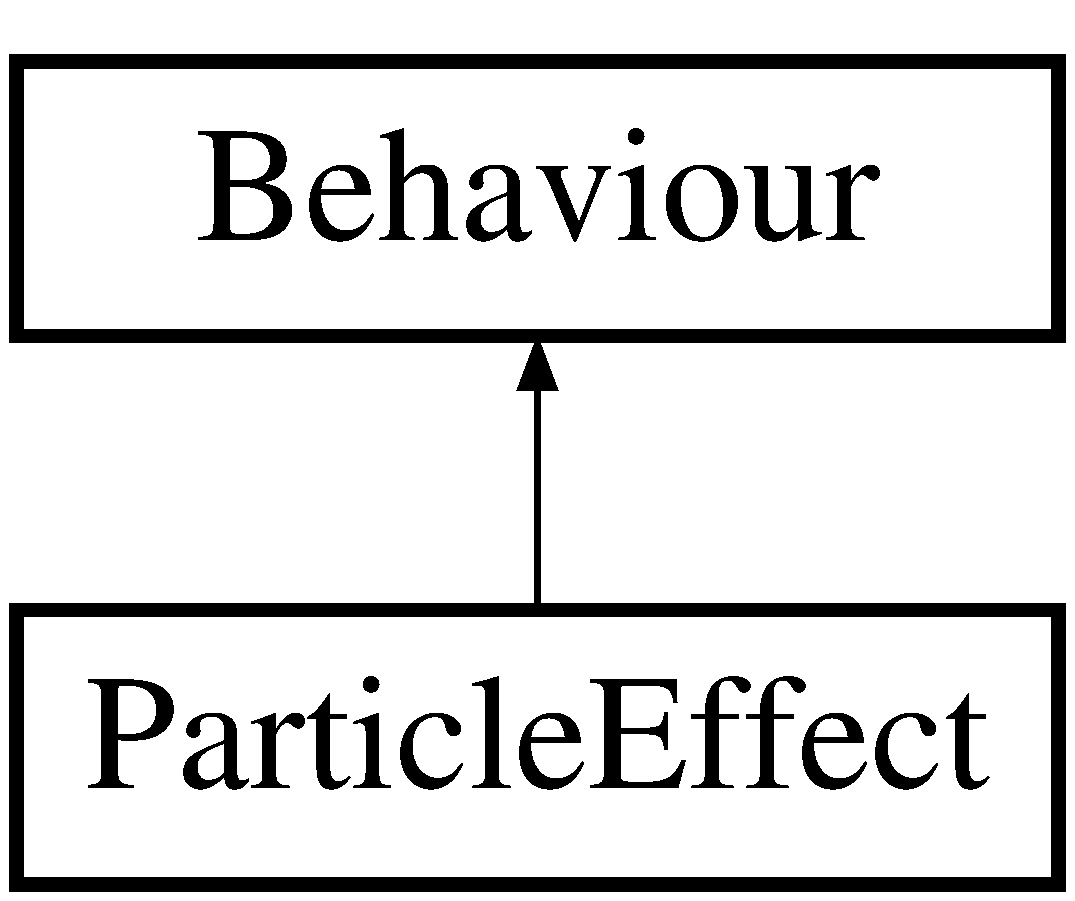
\includegraphics[height=2.000000cm]{class_particle_effect}
\end{center}
\end{figure}
\subsection*{Public Member Functions}
\begin{DoxyCompactItemize}
\item 
\mbox{\Hypertarget{class_particle_effect_a1286fd1a55670af9e1c2c208cef9108e}\label{class_particle_effect_a1286fd1a55670af9e1c2c208cef9108e}} 
void {\bfseries update} ()
\item 
\mbox{\Hypertarget{class_particle_effect_a899030bedb487dbb707b9787ecbe1cb5}\label{class_particle_effect_a899030bedb487dbb707b9787ecbe1cb5}} 
void {\bfseries init} ()
\item 
\mbox{\Hypertarget{class_particle_effect_a252b170dba69a5b8c8c1e1fa6a1b066b}\label{class_particle_effect_a252b170dba69a5b8c8c1e1fa6a1b066b}} 
void {\bfseries set\+Shader} (\hyperlink{class_shader}{Shader} shader)
\end{DoxyCompactItemize}
\subsection*{Additional Inherited Members}


The documentation for this class was generated from the following files\+:\begin{DoxyCompactItemize}
\item 
C\+:/\+Users/szymk/\+Downloads/\+Nowy folder/\+Simple\+Game\+Engine/\+Simple\+Game\+Engine/\+G\+Kp/Particle\+Effect.\+h\item 
C\+:/\+Users/szymk/\+Downloads/\+Nowy folder/\+Simple\+Game\+Engine/\+Simple\+Game\+Engine/\+G\+Kp/Particle\+Effect.\+cpp\end{DoxyCompactItemize}

\hypertarget{class_physical_object}{}\section{Physical\+Object Class Reference}
\label{class_physical_object}\index{Physical\+Object@{Physical\+Object}}


klasa rozszerzajaca klase \hyperlink{class_simple_object}{Simple\+Object} posiada dodatkowe pole opisujace ksztalt oraz wlasciwosci obiektu fizycznego /summary$>$  




{\ttfamily \#include $<$Physical\+Object.\+h$>$}

Inheritance diagram for Physical\+Object\+:\begin{figure}[H]
\begin{center}
\leavevmode
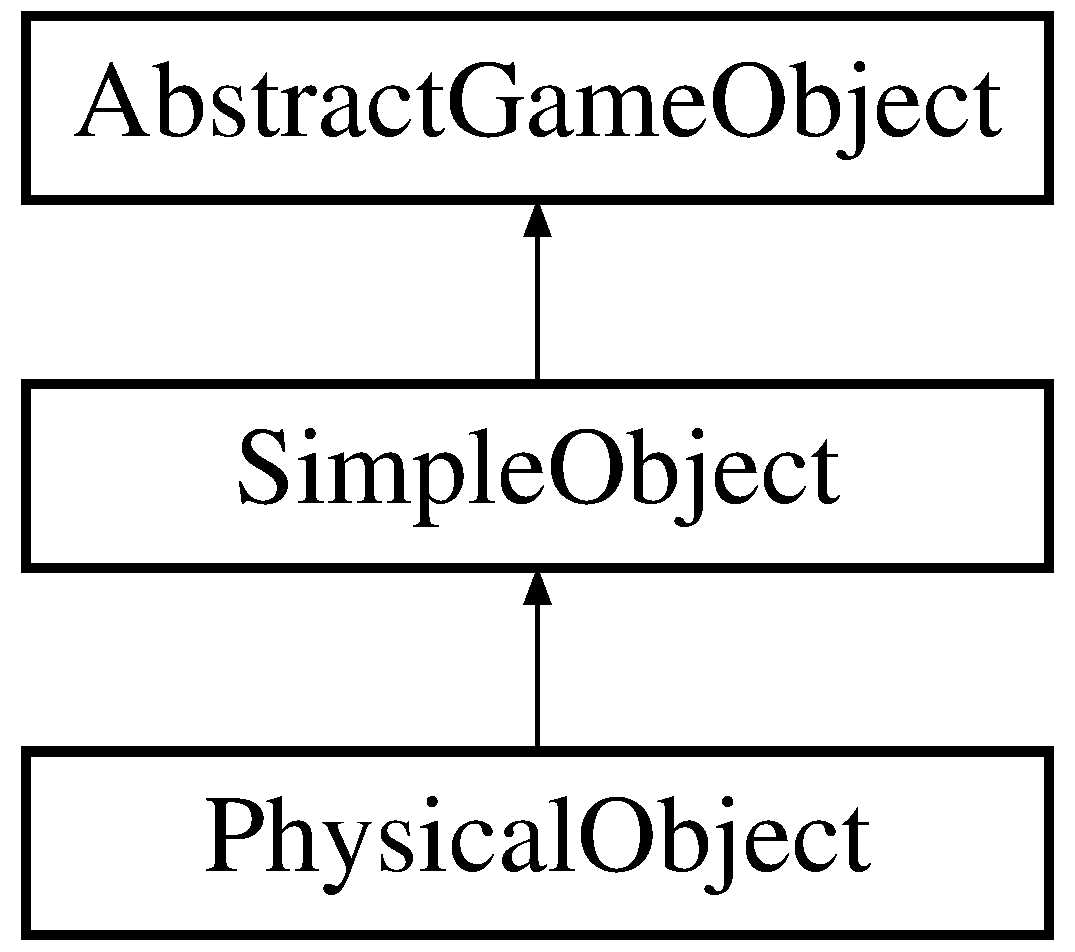
\includegraphics[height=3.000000cm]{class_physical_object}
\end{center}
\end{figure}
\subsection*{Public Member Functions}
\begin{DoxyCompactItemize}
\item 
\mbox{\Hypertarget{class_physical_object_aee54168bb54a6b9c3d340c9f818a7b53}\label{class_physical_object_aee54168bb54a6b9c3d340c9f818a7b53}} 
{\bfseries Physical\+Object} (glm\+::vec3 position, \hyperlink{class_shader}{Shader} $\ast$shader, \hyperlink{class_texture}{Texture} texture, \hyperlink{class_vao_object}{Vao\+Object} $\ast$vao)
\item 
\mbox{\Hypertarget{class_physical_object_a3e3f19518fbd261817e42c5a78fb543d}\label{class_physical_object_a3e3f19518fbd261817e42c5a78fb543d}} 
{\bfseries Physical\+Object} (glm\+::vec3 position, \hyperlink{class_shader}{Shader} $\ast$shader, \hyperlink{class_texture}{Texture} texture, \hyperlink{class_vao_object}{Vao\+Object} $\ast$vao, bt\+Rigid\+Body $\ast$rig\+Body)
\item 
\mbox{\Hypertarget{class_physical_object_af216654d65cdf55b16f1f9da03572dee}\label{class_physical_object_af216654d65cdf55b16f1f9da03572dee}} 
{\bfseries Physical\+Object} (glm\+::vec3 position, \hyperlink{class_shader}{Shader} $\ast$shader, \hyperlink{class_texture}{Texture} texture, \hyperlink{class_vao_object}{Vao\+Object} $\ast$vao, std\+::string rigid\+Body\+Type)
\item 
\mbox{\Hypertarget{class_physical_object_a8e21f75621841ccd58a7cc757fb1c445}\label{class_physical_object_a8e21f75621841ccd58a7cc757fb1c445}} 
{\bfseries Physical\+Object} (glm\+::mat4 transform, \hyperlink{class_shader}{Shader} $\ast$shader, \hyperlink{class_texture}{Texture} texture, \hyperlink{class_vao_object}{Vao\+Object} $\ast$vao, std\+::string rigid\+Body\+Type)
\item 
\mbox{\Hypertarget{class_physical_object_a729b7781a7f7de8dd076f28cca54742f}\label{class_physical_object_a729b7781a7f7de8dd076f28cca54742f}} 
{\bfseries Physical\+Object} (glm\+::vec3 position, \hyperlink{class_shader}{Shader} $\ast$shader, \hyperlink{class_texture}{Texture} texture, \hyperlink{class_vao_object}{Vao\+Object} $\ast$vao, std\+::string rigid\+Body\+Type, glm\+::vec3 dir)
\item 
\mbox{\Hypertarget{class_physical_object_a99886c0d01149e4ab04d9f7598f391db}\label{class_physical_object_a99886c0d01149e4ab04d9f7598f391db}} 
bt\+Rigid\+Body $\ast$ {\bfseries get\+Rigid\+Body} ()
\item 
\mbox{\Hypertarget{class_physical_object_a4aefb72365f6a824a04d0090bfe8c078}\label{class_physical_object_a4aefb72365f6a824a04d0090bfe8c078}} 
void {\bfseries set\+Rigid\+Body} (bt\+Rigid\+Body $\ast$ridig\+Body)
\item 
\mbox{\Hypertarget{class_physical_object_a593d2b001986681081bd39a134788ef8}\label{class_physical_object_a593d2b001986681081bd39a134788ef8}} 
void {\bfseries set\+Collision\+Shape} (bt\+Collision\+Shape $\ast$collision\+Shape)
\item 
void \hyperlink{class_physical_object_a3005ac0afce838049101db17525f6004}{update} ()
\item 
\mbox{\Hypertarget{class_physical_object_a48b1709afb0f331deb7b59e5d98ccdc5}\label{class_physical_object_a48b1709afb0f331deb7b59e5d98ccdc5}} 
virtual void {\bfseries to\+Xml} (X\+M\+L\+Document $\ast$xml\+Doc)
\item 
\mbox{\Hypertarget{class_physical_object_a6148d7d581c15eafa4d8a885719083dc}\label{class_physical_object_a6148d7d581c15eafa4d8a885719083dc}} 
void {\bfseries set\+Rigid\+Body\+Type} (std\+::string type)
\end{DoxyCompactItemize}
\subsection*{Additional Inherited Members}


\subsection{Detailed Description}
klasa rozszerzajaca klase \hyperlink{class_simple_object}{Simple\+Object} posiada dodatkowe pole opisujace ksztalt oraz wlasciwosci obiektu fizycznego /summary$>$ 

\subsection{Member Function Documentation}
\mbox{\Hypertarget{class_physical_object_a3005ac0afce838049101db17525f6004}\label{class_physical_object_a3005ac0afce838049101db17525f6004}} 
\index{Physical\+Object@{Physical\+Object}!update@{update}}
\index{update@{update}!Physical\+Object@{Physical\+Object}}
\subsubsection{\texorpdfstring{update()}{update()}}
{\footnotesize\ttfamily void Physical\+Object\+::update (\begin{DoxyParamCaption}{ }\end{DoxyParamCaption})\hspace{0.3cm}{\ttfamily [virtual]}}

summary$>$ metoda wywolywana co klatke rysujaca obiekt na ekranie /summary$>$ 

Reimplemented from \hyperlink{class_simple_object_a38a3ceafd11a673fd68dd87ed6ebd35b}{Simple\+Object}.



The documentation for this class was generated from the following files\+:\begin{DoxyCompactItemize}
\item 
C\+:/\+Users/szymk/\+Downloads/\+Nowy folder/\+Simple\+Game\+Engine/\+Simple\+Game\+Engine/\+G\+Kp/Physical\+Object.\+h\item 
C\+:/\+Users/szymk/\+Downloads/\+Nowy folder/\+Simple\+Game\+Engine/\+Simple\+Game\+Engine/\+G\+Kp/Physical\+Object.\+cpp\end{DoxyCompactItemize}

\hypertarget{class_physics_world}{}\section{Physics\+World Class Reference}
\label{class_physics_world}\index{Physics\+World@{Physics\+World}}


klasa reprezetujaca fizyczny swiat. /summary$>$  




{\ttfamily \#include $<$Physics\+World.\+h$>$}

\subsection*{Public Member Functions}
\begin{DoxyCompactItemize}
\item 
\hyperlink{class_physics_world_abf1573b008b52b60a83a8f36cbdd51bc}{$\sim$\+Physics\+World} ()
\item 
\mbox{\Hypertarget{class_physics_world_aad64a97f3734de0937f12d665dae7dab}\label{class_physics_world_aad64a97f3734de0937f12d665dae7dab}} 
void {\bfseries init} ()
\item 
void \hyperlink{class_physics_world_aebc88d1b3c209a48c2abf0c8a4aabd51}{update} (double delta\+Time)
\begin{DoxyCompactList}\small\item\em metoda aktualizujaca fizyczny swiat gry o czas podany w parametrze \end{DoxyCompactList}\item 
void \hyperlink{class_physics_world_aa97ff9b7388afe747b447b42aeccfb8c}{add\+Physical\+Object} (\hyperlink{class_physical_object}{Physical\+Object} $\ast$phyobj)
\begin{DoxyCompactList}\small\item\em metoda pozwalajaca na dodanie obiektu fizycznego do swiata fizycznego \end{DoxyCompactList}\item 
\mbox{\Hypertarget{class_physics_world_a9bd79f2fc82a6e50c1ae94719fe9b67f}\label{class_physics_world_a9bd79f2fc82a6e50c1ae94719fe9b67f}} 
void {\bfseries set\+Camera\+Pos} (glm\+::vec3 camera\+Pos)
\item 
\mbox{\Hypertarget{class_physics_world_a6ab733de6f30178a41455d27cd29bf0d}\label{class_physics_world_a6ab733de6f30178a41455d27cd29bf0d}} 
void {\bfseries set\+Camera\+Front} (glm\+::vec3 camera\+Front)
\item 
\mbox{\Hypertarget{class_physics_world_a84a45466593d61dce71666d87edf2038}\label{class_physics_world_a84a45466593d61dce71666d87edf2038}} 
void {\bfseries set\+Rey\+Test\+Obj} (\hyperlink{class_abstract_game_object}{Abstract\+Game\+Object} $\ast$ray\+Test)
\item 
void \hyperlink{class_physics_world_a948724c83bcd3d69a0977b5c9e2b9ac4}{clear} ()
\begin{DoxyCompactList}\small\item\em metoda oczyszczajaca swiat z wszystkich obiektow fizycznych wykorzystywana podczas ladowania wczesniej zapisanego stanu gry \end{DoxyCompactList}\end{DoxyCompactItemize}


\subsection{Detailed Description}
klasa reprezetujaca fizyczny swiat. /summary$>$ 

\subsection{Constructor \& Destructor Documentation}
\mbox{\Hypertarget{class_physics_world_abf1573b008b52b60a83a8f36cbdd51bc}\label{class_physics_world_abf1573b008b52b60a83a8f36cbdd51bc}} 
\index{Physics\+World@{Physics\+World}!````~Physics\+World@{$\sim$\+Physics\+World}}
\index{````~Physics\+World@{$\sim$\+Physics\+World}!Physics\+World@{Physics\+World}}
\subsubsection{\texorpdfstring{$\sim$\+Physics\+World()}{~PhysicsWorld()}}
{\footnotesize\ttfamily Physics\+World\+::$\sim$\+Physics\+World (\begin{DoxyParamCaption}{ }\end{DoxyParamCaption})}

summary$>$ metoda inicjalizujaca fizyczny swiat, ustawia grawitacje /summary$>$ 

\subsection{Member Function Documentation}
\mbox{\Hypertarget{class_physics_world_aa97ff9b7388afe747b447b42aeccfb8c}\label{class_physics_world_aa97ff9b7388afe747b447b42aeccfb8c}} 
\index{Physics\+World@{Physics\+World}!add\+Physical\+Object@{add\+Physical\+Object}}
\index{add\+Physical\+Object@{add\+Physical\+Object}!Physics\+World@{Physics\+World}}
\subsubsection{\texorpdfstring{add\+Physical\+Object()}{addPhysicalObject()}}
{\footnotesize\ttfamily void Physics\+World\+::add\+Physical\+Object (\begin{DoxyParamCaption}\item[{\hyperlink{class_physical_object}{Physical\+Object} $\ast$}]{phyobj }\end{DoxyParamCaption})}



metoda pozwalajaca na dodanie obiektu fizycznego do swiata fizycznego 

\hyperlink{class_physical_object}{Physical\+Object} $\ast$ phyobj -\/ wskaznik na obiekt fizyczny ktory zostanie dodany do fizycznego swiata \mbox{\Hypertarget{class_physics_world_a948724c83bcd3d69a0977b5c9e2b9ac4}\label{class_physics_world_a948724c83bcd3d69a0977b5c9e2b9ac4}} 
\index{Physics\+World@{Physics\+World}!clear@{clear}}
\index{clear@{clear}!Physics\+World@{Physics\+World}}
\subsubsection{\texorpdfstring{clear()}{clear()}}
{\footnotesize\ttfamily void Physics\+World\+::clear (\begin{DoxyParamCaption}{ }\end{DoxyParamCaption})}



metoda oczyszczajaca swiat z wszystkich obiektow fizycznych wykorzystywana podczas ladowania wczesniej zapisanego stanu gry 

\mbox{\Hypertarget{class_physics_world_aebc88d1b3c209a48c2abf0c8a4aabd51}\label{class_physics_world_aebc88d1b3c209a48c2abf0c8a4aabd51}} 
\index{Physics\+World@{Physics\+World}!update@{update}}
\index{update@{update}!Physics\+World@{Physics\+World}}
\subsubsection{\texorpdfstring{update()}{update()}}
{\footnotesize\ttfamily void Physics\+World\+::update (\begin{DoxyParamCaption}\item[{double}]{delta\+Time }\end{DoxyParamCaption})}



metoda aktualizujaca fizyczny swiat gry o czas podany w parametrze 



The documentation for this class was generated from the following files\+:\begin{DoxyCompactItemize}
\item 
C\+:/\+Users/szymk/\+Downloads/\+Nowy folder/\+Simple\+Game\+Engine/\+Simple\+Game\+Engine/\+G\+Kp/Physics\+World.\+h\item 
C\+:/\+Users/szymk/\+Downloads/\+Nowy folder/\+Simple\+Game\+Engine/\+Simple\+Game\+Engine/\+G\+Kp/Physics\+World.\+cpp\end{DoxyCompactItemize}

\hypertarget{class_resource_manager}{}\section{Resource\+Manager Class Reference}
\label{class_resource_manager}\index{Resource\+Manager@{Resource\+Manager}}


statyczna klasa odpowiedzialna za wczytywanie oraz przechowywanie zasob�w takich jak tekstury , shadery oraz siatki(\+Vertex Array Objects). Klasa ta tworzy instancje klas \hyperlink{class_shader}{Shader},\hyperlink{class_texture}{Texture} i \hyperlink{class_vao_object}{Vao\+Object}. /summary$>$  




{\ttfamily \#include $<$Resource\+Manager.\+h$>$}

\subsection*{Static Public Member Functions}
\begin{DoxyCompactItemize}
\item 
static void \hyperlink{class_resource_manager_a21ff03ed8d88126243b33bb75fb308b7}{load\+Shader} (string v\+Shader\+File, string f\+Shader\+File, string name)
\begin{DoxyCompactList}\small\item\em kompiluje shadery z plikow o podanych nazwach i przechowuje ich id w mapie pod kluczem podanym w parametrze name \end{DoxyCompactList}\item 
static void \hyperlink{class_resource_manager_a813e553b7f7df873b455e86ab7445b1c}{load\+Shader} (string v\+Shader\+File, string f\+Shader\+File, string g\+Shader\+File, string name)
\begin{DoxyCompactList}\small\item\em kompiluje shadery z plikow o podanych nazwach i przechowuje ich id w mapie pod kluczem podanym w parametrze name \end{DoxyCompactList}\item 
static \hyperlink{class_shader}{Shader} $\ast$ \hyperlink{class_resource_manager_ae95ecdc6de1127616485f7d069437332}{Get\+Shader} (std\+::string name)
\begin{DoxyCompactList}\small\item\em zwraca shader o kluczu podanym w parametrze \end{DoxyCompactList}\item 
static \hyperlink{class_texture}{Texture} \hyperlink{class_resource_manager_a35ccd9bf812af37f10a17e061402e11f}{Load\+Texture} (const G\+Lchar $\ast$file, G\+Lboolean alpha, string name)
\begin{DoxyCompactList}\small\item\em laduje teksture z pliku podanego w parametrze i zapisuje ja w mapie \end{DoxyCompactList}\item 
\mbox{\Hypertarget{class_resource_manager_a8e1a23eca5474aa435c641666257a255}\label{class_resource_manager_a8e1a23eca5474aa435c641666257a255}} 
static \hyperlink{class_texture}{Texture} {\bfseries Get\+Texture} (std\+::string name)
\item 
\mbox{\Hypertarget{class_resource_manager_abc048e566e7de69db49fb80428bdc8ab}\label{class_resource_manager_abc048e566e7de69db49fb80428bdc8ab}} 
static \hyperlink{class_vao_object}{Vao\+Object} {\bfseries load\+V\+A\+O\+From\+File} (const G\+Lchar $\ast$file, string=\char`\"{}\char`\"{}, bool read\+Normals=false)
\item 
static \hyperlink{class_vao_object}{Vao\+Object} \hyperlink{class_resource_manager_af49529027ae46f78df99bc4f499e1302}{load\+V\+AO} (G\+Lfloat $\ast$vertices\+Array, G\+Luint number\+Of\+Values, bool normals, string name)
\begin{DoxyCompactList}\small\item\em laduje V\+AO z pliku podanego w parametrze i zapisuje je w mapie \end{DoxyCompactList}\item 
\mbox{\Hypertarget{class_resource_manager_a23ec806a48cf4d277742f54bfc7a4c0c}\label{class_resource_manager_a23ec806a48cf4d277742f54bfc7a4c0c}} 
static \hyperlink{class_vao_object}{Vao\+Object} $\ast$ {\bfseries get\+V\+AO} (string name)
\item 
static void \hyperlink{class_resource_manager_a8d5a441251bf579b25ff3ab3e7c28342}{delete\+Assets} ()
\begin{DoxyCompactList}\small\item\em usowa zasoby z kolekcji \end{DoxyCompactList}\item 
static unsigned int \hyperlink{class_resource_manager_ad311e01ff4231f57b210cdf8342210c7}{load\+Cubemap} (vector$<$ std\+::string $>$ faces)
\begin{DoxyCompactList}\small\item\em laduje tekstury skyboxa z pliku i tworzy z nich skyboxa \end{DoxyCompactList}\item 
\mbox{\Hypertarget{class_resource_manager_ad8cdb632b2b69e791e82aa3f66c135e6}\label{class_resource_manager_ad8cdb632b2b69e791e82aa3f66c135e6}} 
static bool {\bfseries read\+World} (std\+::string wordl\+Name)
\item 
\mbox{\Hypertarget{class_resource_manager_abeb131a622f64d59c938fd238d3802f8}\label{class_resource_manager_abeb131a622f64d59c938fd238d3802f8}} 
static std\+::vector$<$ std\+::string $>$ {\bfseries Get\+Texture\+Names} ()
\end{DoxyCompactItemize}


\subsection{Detailed Description}
statyczna klasa odpowiedzialna za wczytywanie oraz przechowywanie zasob�w takich jak tekstury , shadery oraz siatki(\+Vertex Array Objects). Klasa ta tworzy instancje klas \hyperlink{class_shader}{Shader},\hyperlink{class_texture}{Texture} i \hyperlink{class_vao_object}{Vao\+Object}. /summary$>$ 

\subsection{Member Function Documentation}
\mbox{\Hypertarget{class_resource_manager_a8d5a441251bf579b25ff3ab3e7c28342}\label{class_resource_manager_a8d5a441251bf579b25ff3ab3e7c28342}} 
\index{Resource\+Manager@{Resource\+Manager}!delete\+Assets@{delete\+Assets}}
\index{delete\+Assets@{delete\+Assets}!Resource\+Manager@{Resource\+Manager}}
\subsubsection{\texorpdfstring{delete\+Assets()}{deleteAssets()}}
{\footnotesize\ttfamily void Resource\+Manager\+::delete\+Assets (\begin{DoxyParamCaption}{ }\end{DoxyParamCaption})\hspace{0.3cm}{\ttfamily [static]}}



usowa zasoby z kolekcji 

\mbox{\Hypertarget{class_resource_manager_ae95ecdc6de1127616485f7d069437332}\label{class_resource_manager_ae95ecdc6de1127616485f7d069437332}} 
\index{Resource\+Manager@{Resource\+Manager}!Get\+Shader@{Get\+Shader}}
\index{Get\+Shader@{Get\+Shader}!Resource\+Manager@{Resource\+Manager}}
\subsubsection{\texorpdfstring{Get\+Shader()}{GetShader()}}
{\footnotesize\ttfamily \hyperlink{class_shader}{Shader} $\ast$ Resource\+Manager\+::\+Get\+Shader (\begin{DoxyParamCaption}\item[{std\+::string}]{name }\end{DoxyParamCaption})\hspace{0.3cm}{\ttfamily [static]}}



zwraca shader o kluczu podanym w parametrze 

\mbox{\Hypertarget{class_resource_manager_ad311e01ff4231f57b210cdf8342210c7}\label{class_resource_manager_ad311e01ff4231f57b210cdf8342210c7}} 
\index{Resource\+Manager@{Resource\+Manager}!load\+Cubemap@{load\+Cubemap}}
\index{load\+Cubemap@{load\+Cubemap}!Resource\+Manager@{Resource\+Manager}}
\subsubsection{\texorpdfstring{load\+Cubemap()}{loadCubemap()}}
{\footnotesize\ttfamily unsigned int Resource\+Manager\+::load\+Cubemap (\begin{DoxyParamCaption}\item[{vector$<$ std\+::string $>$}]{faces }\end{DoxyParamCaption})\hspace{0.3cm}{\ttfamily [static]}}



laduje tekstury skyboxa z pliku i tworzy z nich skyboxa 

vector$<$std\+::string$>$ faces -\/ wektor przechowujacy obrazki z ktorych ma zostac zbudowany skybox \mbox{\Hypertarget{class_resource_manager_a21ff03ed8d88126243b33bb75fb308b7}\label{class_resource_manager_a21ff03ed8d88126243b33bb75fb308b7}} 
\index{Resource\+Manager@{Resource\+Manager}!load\+Shader@{load\+Shader}}
\index{load\+Shader@{load\+Shader}!Resource\+Manager@{Resource\+Manager}}
\subsubsection{\texorpdfstring{load\+Shader()}{loadShader()}\hspace{0.1cm}{\footnotesize\ttfamily [1/2]}}
{\footnotesize\ttfamily void Resource\+Manager\+::load\+Shader (\begin{DoxyParamCaption}\item[{string}]{v\+Shader\+File,  }\item[{string}]{f\+Shader\+File,  }\item[{string}]{name }\end{DoxyParamCaption})\hspace{0.3cm}{\ttfamily [static]}}



kompiluje shadery z plikow o podanych nazwach i przechowuje ich id w mapie pod kluczem podanym w parametrze name 

\mbox{\Hypertarget{class_resource_manager_a813e553b7f7df873b455e86ab7445b1c}\label{class_resource_manager_a813e553b7f7df873b455e86ab7445b1c}} 
\index{Resource\+Manager@{Resource\+Manager}!load\+Shader@{load\+Shader}}
\index{load\+Shader@{load\+Shader}!Resource\+Manager@{Resource\+Manager}}
\subsubsection{\texorpdfstring{load\+Shader()}{loadShader()}\hspace{0.1cm}{\footnotesize\ttfamily [2/2]}}
{\footnotesize\ttfamily void Resource\+Manager\+::load\+Shader (\begin{DoxyParamCaption}\item[{string}]{v\+Shader\+File,  }\item[{string}]{f\+Shader\+File,  }\item[{string}]{g\+Shader\+File,  }\item[{string}]{name }\end{DoxyParamCaption})\hspace{0.3cm}{\ttfamily [static]}}



kompiluje shadery z plikow o podanych nazwach i przechowuje ich id w mapie pod kluczem podanym w parametrze name 

\mbox{\Hypertarget{class_resource_manager_a35ccd9bf812af37f10a17e061402e11f}\label{class_resource_manager_a35ccd9bf812af37f10a17e061402e11f}} 
\index{Resource\+Manager@{Resource\+Manager}!Load\+Texture@{Load\+Texture}}
\index{Load\+Texture@{Load\+Texture}!Resource\+Manager@{Resource\+Manager}}
\subsubsection{\texorpdfstring{Load\+Texture()}{LoadTexture()}}
{\footnotesize\ttfamily \hyperlink{class_texture}{Texture} Resource\+Manager\+::\+Load\+Texture (\begin{DoxyParamCaption}\item[{const G\+Lchar $\ast$}]{file,  }\item[{G\+Lboolean}]{alpha,  }\item[{string}]{name }\end{DoxyParamCaption})\hspace{0.3cm}{\ttfamily [static]}}



laduje teksture z pliku podanego w parametrze i zapisuje ja w mapie 

param$>$ string name -\/ klucz pod ktorym zostanie zapisana tekstura /param$>$ \mbox{\Hypertarget{class_resource_manager_af49529027ae46f78df99bc4f499e1302}\label{class_resource_manager_af49529027ae46f78df99bc4f499e1302}} 
\index{Resource\+Manager@{Resource\+Manager}!load\+V\+AO@{load\+V\+AO}}
\index{load\+V\+AO@{load\+V\+AO}!Resource\+Manager@{Resource\+Manager}}
\subsubsection{\texorpdfstring{load\+V\+A\+O()}{loadVAO()}}
{\footnotesize\ttfamily \hyperlink{class_vao_object}{Vao\+Object} Resource\+Manager\+::load\+V\+AO (\begin{DoxyParamCaption}\item[{G\+Lfloat $\ast$}]{vertices\+Array,  }\item[{G\+Luint}]{number\+Of\+Values,  }\item[{bool}]{normals,  }\item[{string}]{name }\end{DoxyParamCaption})\hspace{0.3cm}{\ttfamily [static]}}



laduje V\+AO z pliku podanego w parametrze i zapisuje je w mapie 

string name -\/ klucz pod ktorym zostanie zapisane V\+AO 

The documentation for this class was generated from the following files\+:\begin{DoxyCompactItemize}
\item 
C\+:/\+Users/szymk/\+Downloads/\+Nowy folder/\+Simple\+Game\+Engine/\+Simple\+Game\+Engine/\+G\+Kp/Resource\+Manager.\+h\item 
C\+:/\+Users/szymk/\+Downloads/\+Nowy folder/\+Simple\+Game\+Engine/\+Simple\+Game\+Engine/\+G\+Kp/Game.\+cpp\item 
C\+:/\+Users/szymk/\+Downloads/\+Nowy folder/\+Simple\+Game\+Engine/\+Simple\+Game\+Engine/\+G\+Kp/Resource\+Manager.\+cpp\end{DoxyCompactItemize}

\hypertarget{class_rigid_body_simple_factory}{}\section{Rigid\+Body\+Simple\+Factory Class Reference}
\label{class_rigid_body_simple_factory}\index{Rigid\+Body\+Simple\+Factory@{Rigid\+Body\+Simple\+Factory}}


klasa odpowiadajaca za tworzenie cial fizycznych /summary$>$  




{\ttfamily \#include $<$Rigid\+Body\+Simple\+Factory.\+h$>$}

\subsection*{Static Public Member Functions}
\begin{DoxyCompactItemize}
\item 
\mbox{\Hypertarget{class_rigid_body_simple_factory_a69c29aeb05d934766c3ae082c48efe2f}\label{class_rigid_body_simple_factory_a69c29aeb05d934766c3ae082c48efe2f}} 
static bt\+Rigid\+Body $\ast$ {\bfseries create\+Rigid\+Body} (std\+::string type, bt\+Transform tr)
\end{DoxyCompactItemize}


\subsection{Detailed Description}
klasa odpowiadajaca za tworzenie cial fizycznych /summary$>$ 

The documentation for this class was generated from the following files\+:\begin{DoxyCompactItemize}
\item 
C\+:/\+Users/szymk/\+Downloads/\+Nowy folder/\+Simple\+Game\+Engine/\+Simple\+Game\+Engine/\+G\+Kp/Rigid\+Body\+Simple\+Factory.\+h\item 
C\+:/\+Users/szymk/\+Downloads/\+Nowy folder/\+Simple\+Game\+Engine/\+Simple\+Game\+Engine/\+G\+Kp/Rigid\+Body\+Simple\+Factory.\+cpp\end{DoxyCompactItemize}

\hypertarget{class_shader}{}\section{Shader Class Reference}
\label{class_shader}\index{Shader@{Shader}}


klasa umo�liwiaj�ca kompilacje shaderow. Przechowywane w polu numer ID shadera. Posiada metod� use() kt�ra wywo�uje funkcj� gl\+Use\+Program dla ID przechowywanego w polu obiektu.  




{\ttfamily \#include $<$Shader.\+h$>$}

\subsection*{Public Member Functions}
\begin{DoxyCompactItemize}
\item 
\mbox{\Hypertarget{class_shader_ad1bc9a16400499ec80c4f716a390abaf}\label{class_shader_ad1bc9a16400499ec80c4f716a390abaf}} 
G\+Luint {\bfseries get\+ID} ()
\item 
\mbox{\Hypertarget{class_shader_aaac878c2f54bbf976169fca353aef9dc}\label{class_shader_aaac878c2f54bbf976169fca353aef9dc}} 
void {\bfseries compile} (const G\+Lchar $\ast$vs\+Source, const G\+Lchar $\ast$fs\+Source, const G\+Lchar $\ast$gs\+Source=\char`\"{}\char`\"{})
\item 
\mbox{\Hypertarget{class_shader_ac5ed889fa0a460c727557a9c0868cf55}\label{class_shader_ac5ed889fa0a460c727557a9c0868cf55}} 
\hyperlink{class_shader}{Shader} \& {\bfseries use} ()
\item 
\mbox{\Hypertarget{class_shader_a7982747baa5d27f1f533b995e584c939}\label{class_shader_a7982747baa5d27f1f533b995e584c939}} 
std\+::string {\bfseries get\+Name} ()
\item 
\mbox{\Hypertarget{class_shader_adffdcd0c5109ad65a5acdd926b28bbb0}\label{class_shader_adffdcd0c5109ad65a5acdd926b28bbb0}} 
void {\bfseries set\+Name} (std\+::string name)
\end{DoxyCompactItemize}


\subsection{Detailed Description}
klasa umo�liwiaj�ca kompilacje shaderow. Przechowywane w polu numer ID shadera. Posiada metod� use() kt�ra wywo�uje funkcj� gl\+Use\+Program dla ID przechowywanego w polu obiektu. 

/summary$>$ 

The documentation for this class was generated from the following files\+:\begin{DoxyCompactItemize}
\item 
C\+:/\+Users/szymk/\+Downloads/\+Nowy folder/\+Simple\+Game\+Engine/\+Simple\+Game\+Engine/\+G\+Kp/Shader.\+h\item 
C\+:/\+Users/szymk/\+Downloads/\+Nowy folder/\+Simple\+Game\+Engine/\+Simple\+Game\+Engine/\+G\+Kp/Shader.\+cpp\end{DoxyCompactItemize}

\hypertarget{class_simple_object}{}\section{Simple\+Object Class Reference}
\label{class_simple_object}\index{Simple\+Object@{Simple\+Object}}


klasa implementujaca \hyperlink{class_abstract_game_object}{Abstract\+Game\+Object}. Reprezetuje podstawowy obiekt gry nie posiadajacy wlasciwosci fizycznych /summary$>$  




{\ttfamily \#include $<$Simple\+Object.\+h$>$}

Inheritance diagram for Simple\+Object\+:\begin{figure}[H]
\begin{center}
\leavevmode
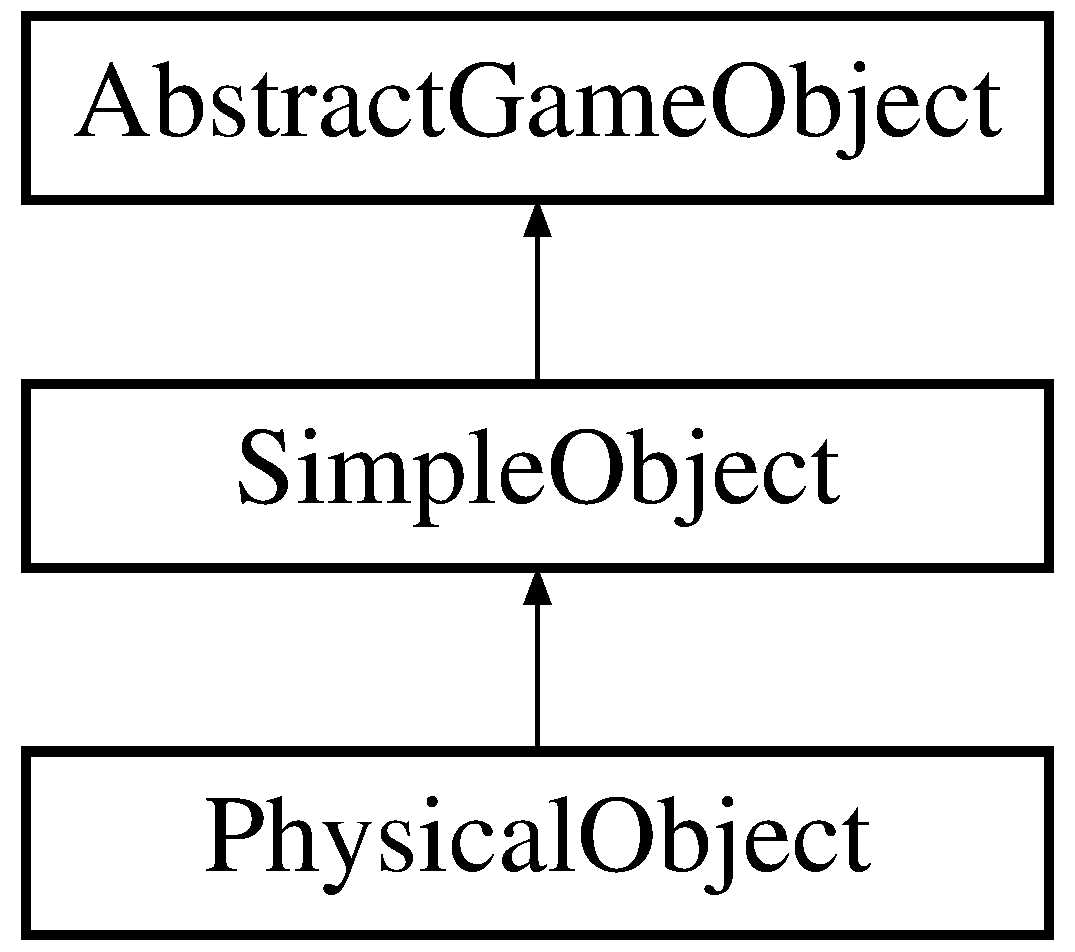
\includegraphics[height=3.000000cm]{class_simple_object}
\end{center}
\end{figure}
\subsection*{Public Member Functions}
\begin{DoxyCompactItemize}
\item 
\mbox{\Hypertarget{class_simple_object_a4b237a7f96bed83ec599c0af41a9dbf6}\label{class_simple_object_a4b237a7f96bed83ec599c0af41a9dbf6}} 
{\bfseries Simple\+Object} (glm\+::vec3 position, \hyperlink{class_shader}{Shader} $\ast$shader, \hyperlink{class_texture}{Texture} texture, \hyperlink{class_vao_object}{Vao\+Object} $\ast$vao)
\item 
\mbox{\Hypertarget{class_simple_object_ad0d7d8b5224adfb044be1a9a11dbdda8}\label{class_simple_object_ad0d7d8b5224adfb044be1a9a11dbdda8}} 
{\bfseries Simple\+Object} (glm\+::mat4 transform, \hyperlink{class_shader}{Shader} $\ast$shader, \hyperlink{class_texture}{Texture} texture, \hyperlink{class_vao_object}{Vao\+Object} $\ast$vao)
\item 
\mbox{\Hypertarget{class_simple_object_a24bfa1fa17d1097cb197f6350862c39f}\label{class_simple_object_a24bfa1fa17d1097cb197f6350862c39f}} 
{\bfseries Simple\+Object} (glm\+::vec3 position)
\item 
\mbox{\Hypertarget{class_simple_object_a59ed585f31accdf25d14dedbe3463d93}\label{class_simple_object_a59ed585f31accdf25d14dedbe3463d93}} 
{\bfseries Simple\+Object} (\hyperlink{class_texture}{Texture} texture, glm\+::mat4 model\+Matrix, \hyperlink{class_vao_object}{Vao\+Object} $\ast$V\+AO)
\item 
virtual void \hyperlink{class_simple_object_a38a3ceafd11a673fd68dd87ed6ebd35b}{update} ()
\item 
\mbox{\Hypertarget{class_simple_object_a920aa438e4414745847cf284ca00e71d}\label{class_simple_object_a920aa438e4414745847cf284ca00e71d}} 
virtual void {\bfseries draw} ()
\item 
\mbox{\Hypertarget{class_simple_object_aa4d4ccdd87ff9ee1676573e6a1f8a335}\label{class_simple_object_aa4d4ccdd87ff9ee1676573e6a1f8a335}} 
virtual void {\bfseries set\+Shader} (\hyperlink{class_shader}{Shader} $\ast$shader)
\item 
\mbox{\Hypertarget{class_simple_object_a23f24ff02b60e625170e7c00991eeff6}\label{class_simple_object_a23f24ff02b60e625170e7c00991eeff6}} 
void {\bfseries set\+Texture} (\hyperlink{class_texture}{Texture} texture)
\item 
\mbox{\Hypertarget{class_simple_object_a87e1ea0f304176fdb6b61fdd50acedcb}\label{class_simple_object_a87e1ea0f304176fdb6b61fdd50acedcb}} 
void {\bfseries set\+Vao} (\hyperlink{class_vao_object}{Vao\+Object} $\ast$vao)
\item 
\mbox{\Hypertarget{class_simple_object_af6c38301b53a5dd83f38219a62dd5c61}\label{class_simple_object_af6c38301b53a5dd83f38219a62dd5c61}} 
virtual void {\bfseries set\+Position} (glm\+::vec3 position)
\item 
virtual glm\+::vec3 \hyperlink{class_simple_object_acaf96b4cf35863ca69a123d9404f4e5f}{get\+Position} ()
\item 
\mbox{\Hypertarget{class_simple_object_a2a4eba5cc71f93824b66d9b1669032e2}\label{class_simple_object_a2a4eba5cc71f93824b66d9b1669032e2}} 
virtual void {\bfseries set\+Visible} (bool visible)
\item 
virtual bool \hyperlink{class_simple_object_a2475d0a90f1cb7bc5765a632efe9ddd4}{is\+Visible} ()
\item 
\mbox{\Hypertarget{class_simple_object_ad4473aa5bb43047e70b3de73db5c0471}\label{class_simple_object_ad4473aa5bb43047e70b3de73db5c0471}} 
virtual void {\bfseries add\+Behaviour} (\hyperlink{class_behaviour}{Behaviour} $\ast$behaviour)
\item 
\mbox{\Hypertarget{class_simple_object_a89467e4932063b53734ac0e0ff5c05eb}\label{class_simple_object_a89467e4932063b53734ac0e0ff5c05eb}} 
virtual void {\bfseries to\+Xml} (X\+M\+L\+Document $\ast$xml\+Doc)
\end{DoxyCompactItemize}
\subsection*{Protected Member Functions}
\begin{DoxyCompactItemize}
\item 
\mbox{\Hypertarget{class_simple_object_aa6790553dc4f308a99e35ab1f8ad0a64}\label{class_simple_object_aa6790553dc4f308a99e35ab1f8ad0a64}} 
virtual void {\bfseries set\+V\+AO} (\hyperlink{class_vao_object}{Vao\+Object} $\ast$V\+AO)
\item 
\mbox{\Hypertarget{class_simple_object_a906ee1d2032b6f25fdc8eedabf4ac943}\label{class_simple_object_a906ee1d2032b6f25fdc8eedabf4ac943}} 
virtual void {\bfseries set\+Model\+Matrix} (glm\+::mat4 model\+Matrix)
\item 
\mbox{\Hypertarget{class_simple_object_af9aca9384bdda21372ab0f28f02af499}\label{class_simple_object_af9aca9384bdda21372ab0f28f02af499}} 
void {\bfseries model\+Matrix\+To\+Xml} (X\+M\+L\+Element $\ast$matrix)
\end{DoxyCompactItemize}
\subsection*{Protected Attributes}
\begin{DoxyCompactItemize}
\item 
\mbox{\Hypertarget{class_simple_object_afb4e75c108263067f5347198a5e1d890}\label{class_simple_object_afb4e75c108263067f5347198a5e1d890}} 
glm\+::mat4 {\bfseries model\+Matrix}
\item 
\mbox{\Hypertarget{class_simple_object_aa2c839c6fd33d925ffe37949c2f365a8}\label{class_simple_object_aa2c839c6fd33d925ffe37949c2f365a8}} 
\hyperlink{class_shader}{Shader} $\ast$ {\bfseries shader}
\item 
\mbox{\Hypertarget{class_simple_object_a8339746daf36763a8a4312a19ff123de}\label{class_simple_object_a8339746daf36763a8a4312a19ff123de}} 
\hyperlink{class_vao_object}{Vao\+Object} $\ast$ {\bfseries vao}
\item 
\mbox{\Hypertarget{class_simple_object_af94137a8b0e4e71adba0a828263f523a}\label{class_simple_object_af94137a8b0e4e71adba0a828263f523a}} 
\hyperlink{class_texture}{Texture} {\bfseries texture}
\item 
\mbox{\Hypertarget{class_simple_object_ac47c5390bef50cb4b852119274b66ab9}\label{class_simple_object_ac47c5390bef50cb4b852119274b66ab9}} 
std\+::list$<$ \hyperlink{class_behaviour}{Behaviour} $\ast$ $>$ {\bfseries behaviours}
\end{DoxyCompactItemize}


\subsection{Detailed Description}
klasa implementujaca \hyperlink{class_abstract_game_object}{Abstract\+Game\+Object}. Reprezetuje podstawowy obiekt gry nie posiadajacy wlasciwosci fizycznych /summary$>$ 

\subsection{Member Function Documentation}
\mbox{\Hypertarget{class_simple_object_acaf96b4cf35863ca69a123d9404f4e5f}\label{class_simple_object_acaf96b4cf35863ca69a123d9404f4e5f}} 
\index{Simple\+Object@{Simple\+Object}!get\+Position@{get\+Position}}
\index{get\+Position@{get\+Position}!Simple\+Object@{Simple\+Object}}
\subsubsection{\texorpdfstring{get\+Position()}{getPosition()}}
{\footnotesize\ttfamily glm\+::vec3 Simple\+Object\+::get\+Position (\begin{DoxyParamCaption}{ }\end{DoxyParamCaption})\hspace{0.3cm}{\ttfamily [virtual]}}

summary$>$ metoda wywolywana co klatke aktualizujaca stan obiektu /summary$>$ 

Implements \hyperlink{class_abstract_game_object_ac934d513fd18a520d8b68dd5a7ac7399}{Abstract\+Game\+Object}.

\mbox{\Hypertarget{class_simple_object_a2475d0a90f1cb7bc5765a632efe9ddd4}\label{class_simple_object_a2475d0a90f1cb7bc5765a632efe9ddd4}} 
\index{Simple\+Object@{Simple\+Object}!is\+Visible@{is\+Visible}}
\index{is\+Visible@{is\+Visible}!Simple\+Object@{Simple\+Object}}
\subsubsection{\texorpdfstring{is\+Visible()}{isVisible()}}
{\footnotesize\ttfamily bool Simple\+Object\+::is\+Visible (\begin{DoxyParamCaption}{ }\end{DoxyParamCaption})\hspace{0.3cm}{\ttfamily [virtual]}}

summary$>$ metoda dodajaca fragment bedacy opisem obiektu jako X\+ML do dokumentu na ktory wskaznik podawany jest w parametrze /summary$>$ 

Implements \hyperlink{class_abstract_game_object_afddc4040f2d1a7effc0e0baa9950b2e2}{Abstract\+Game\+Object}.

\mbox{\Hypertarget{class_simple_object_a38a3ceafd11a673fd68dd87ed6ebd35b}\label{class_simple_object_a38a3ceafd11a673fd68dd87ed6ebd35b}} 
\index{Simple\+Object@{Simple\+Object}!update@{update}}
\index{update@{update}!Simple\+Object@{Simple\+Object}}
\subsubsection{\texorpdfstring{update()}{update()}}
{\footnotesize\ttfamily void Simple\+Object\+::update (\begin{DoxyParamCaption}{ }\end{DoxyParamCaption})\hspace{0.3cm}{\ttfamily [virtual]}}

summary$>$ metoda wywolywana co klatke rysujaca obiekt na ekranie /summary$>$ 

Implements \hyperlink{class_abstract_game_object_a162f800603ac5671ff24ad8042c062b5}{Abstract\+Game\+Object}.



Reimplemented in \hyperlink{class_physical_object_a3005ac0afce838049101db17525f6004}{Physical\+Object}.



The documentation for this class was generated from the following files\+:\begin{DoxyCompactItemize}
\item 
C\+:/\+Users/szymk/\+Downloads/\+Nowy folder/\+Simple\+Game\+Engine/\+Simple\+Game\+Engine/\+G\+Kp/Simple\+Object.\+h\item 
C\+:/\+Users/szymk/\+Downloads/\+Nowy folder/\+Simple\+Game\+Engine/\+Simple\+Game\+Engine/\+G\+Kp/Simple\+Object.\+cpp\end{DoxyCompactItemize}

\hypertarget{class_texture}{}\section{Texture Class Reference}
\label{class_texture}\index{Texture@{Texture}}


Klasa umo�liwiaj�ca generowanie tekstury na podstawie obrazu. Przechowywuj� w polu ID tekstury oraz informacje o teksturze takie jak rozmiar, wrap, filter. /summary$>$  




{\ttfamily \#include $<$Texture.\+h$>$}

\subsection*{Public Member Functions}
\begin{DoxyCompactItemize}
\item 
\mbox{\Hypertarget{class_texture_aef21ecbdb036febb0840fc7226a1fa36}\label{class_texture_aef21ecbdb036febb0840fc7226a1fa36}} 
void {\bfseries Generate} (G\+Luint width, G\+Luint height, unsigned char $\ast$data)
\item 
\mbox{\Hypertarget{class_texture_a4b85391c6e54686ec566ba38c62dde98}\label{class_texture_a4b85391c6e54686ec566ba38c62dde98}} 
void {\bfseries bind} () const
\item 
\mbox{\Hypertarget{class_texture_ae7ce037f4581332db02ea9efab6cf09a}\label{class_texture_ae7ce037f4581332db02ea9efab6cf09a}} 
void {\bfseries set\+Img\+Format} (G\+Luint img\+Format)
\item 
\mbox{\Hypertarget{class_texture_a97b771df56be41cdaf94cb456cf55506}\label{class_texture_a97b771df56be41cdaf94cb456cf55506}} 
void {\bfseries set\+Int\+Format} (G\+Luint int\+Format)
\item 
\mbox{\Hypertarget{class_texture_a8c80ba7f76f3c9e06e9f83ef0e5f2f49}\label{class_texture_a8c80ba7f76f3c9e06e9f83ef0e5f2f49}} 
G\+Luint {\bfseries get\+Img\+Format} ()
\item 
\mbox{\Hypertarget{class_texture_a2d595785445e26e229e990b2909e4b21}\label{class_texture_a2d595785445e26e229e990b2909e4b21}} 
G\+Luint {\bfseries get\+Int\+Format} ()
\item 
\mbox{\Hypertarget{class_texture_a3fcc1f10d3416dd54c8f0c02d9cd2713}\label{class_texture_a3fcc1f10d3416dd54c8f0c02d9cd2713}} 
G\+Luint {\bfseries get\+ID} ()
\item 
\mbox{\Hypertarget{class_texture_a352ad6a6a3e6d7a7226d95b7612e5d24}\label{class_texture_a352ad6a6a3e6d7a7226d95b7612e5d24}} 
std\+::string {\bfseries get\+Name} ()
\item 
\mbox{\Hypertarget{class_texture_a68c23a1688a28cc07c213e0891fd3a3c}\label{class_texture_a68c23a1688a28cc07c213e0891fd3a3c}} 
void {\bfseries set\+Name} (std\+::string name)
\end{DoxyCompactItemize}


\subsection{Detailed Description}
Klasa umo�liwiaj�ca generowanie tekstury na podstawie obrazu. Przechowywuj� w polu ID tekstury oraz informacje o teksturze takie jak rozmiar, wrap, filter. /summary$>$ 

The documentation for this class was generated from the following files\+:\begin{DoxyCompactItemize}
\item 
C\+:/\+Users/szymk/\+Downloads/\+Nowy folder/\+Simple\+Game\+Engine/\+Simple\+Game\+Engine/\+G\+Kp/Texture.\+h\item 
C\+:/\+Users/szymk/\+Downloads/\+Nowy folder/\+Simple\+Game\+Engine/\+Simple\+Game\+Engine/\+G\+Kp/Texture.\+cpp\end{DoxyCompactItemize}

\hypertarget{class_vao_object}{}\section{Vao\+Object Class Reference}
\label{class_vao_object}\index{Vao\+Object@{Vao\+Object}}


Klasa ta umo�liwia generowanie Vao na podstawie tablicy wierzcho�k�w. W tablicy wierzcho�k�w przechowywane s� ich wsp�rz�dne, wsp�rz�dne tekstur oraz opcjonalnie normalne wierzcho�k�w. Klasa posiada pole przechowuj�ce id wygenerowanego V\+AO. 




{\ttfamily \#include $<$Vao\+Object.\+h$>$}

\subsection*{Public Member Functions}
\begin{DoxyCompactItemize}
\item 
\mbox{\Hypertarget{class_vao_object_a3b4f8a5a57d3e59f23abc33e06250ebf}\label{class_vao_object_a3b4f8a5a57d3e59f23abc33e06250ebf}} 
{\bfseries Vao\+Object} (G\+Lfloat $\ast$vertices\+Array, G\+Luint number\+Of\+Values, bool normals)
\item 
\mbox{\Hypertarget{class_vao_object_a3fe5ae7ae2d8c77c9784ad9ae3e8b851}\label{class_vao_object_a3fe5ae7ae2d8c77c9784ad9ae3e8b851}} 
void {\bfseries generate} (G\+Lfloat $\ast$vertices\+Array, G\+Luint number\+Of\+Values)
\item 
\mbox{\Hypertarget{class_vao_object_a1917ec4ca3cb805bb445b839d06ad4f8}\label{class_vao_object_a1917ec4ca3cb805bb445b839d06ad4f8}} 
G\+Luint {\bfseries get\+ID} ()
\item 
\mbox{\Hypertarget{class_vao_object_adcafdb8b593d62bfb59d2e7da3010644}\label{class_vao_object_adcafdb8b593d62bfb59d2e7da3010644}} 
G\+Luint {\bfseries get\+Triangles\+Number} ()
\item 
\mbox{\Hypertarget{class_vao_object_accbfbb90172347b7d2fd2769584c1fd9}\label{class_vao_object_accbfbb90172347b7d2fd2769584c1fd9}} 
void {\bfseries bind} ()
\item 
\mbox{\Hypertarget{class_vao_object_aabc290cfbc06cc601ac1e23da15ff20d}\label{class_vao_object_aabc290cfbc06cc601ac1e23da15ff20d}} 
std\+::string {\bfseries get\+Name} ()
\item 
\mbox{\Hypertarget{class_vao_object_a1619bfec8f43d1f0db13faa18f405513}\label{class_vao_object_a1619bfec8f43d1f0db13faa18f405513}} 
void {\bfseries set\+Name} (std\+::string name)
\end{DoxyCompactItemize}


\subsection{Detailed Description}
Klasa ta umo�liwia generowanie Vao na podstawie tablicy wierzcho�k�w. W tablicy wierzcho�k�w przechowywane s� ich wsp�rz�dne, wsp�rz�dne tekstur oraz opcjonalnie normalne wierzcho�k�w. Klasa posiada pole przechowuj�ce id wygenerowanego V\+AO.



The documentation for this class was generated from the following files\+:\begin{DoxyCompactItemize}
\item 
C\+:/\+Users/szymk/\+Downloads/\+Nowy folder/\+Simple\+Game\+Engine/\+Simple\+Game\+Engine/\+G\+Kp/Vao\+Object.\+h\item 
C\+:/\+Users/szymk/\+Downloads/\+Nowy folder/\+Simple\+Game\+Engine/\+Simple\+Game\+Engine/\+G\+Kp/Vao\+Object.\+cpp\end{DoxyCompactItemize}

%--- End generated contents ---

% Index
\backmatter
\newpage
\phantomsection
\clearemptydoublepage
\addcontentsline{toc}{chapter}{Index}
\printindex

\end{document}
